En este capítulo, se detalla el plan para implementar y poner en funcionamiento el software del brazo robótico.
\section{Plan de implantación}

La aplicación se ha concebido con la premisa de ser accesible, por lo tanto:
\begin{enumerate}
    \item Se debe descargar.
    \item Se debe descomprimir.
    \item Utilizar.
\end{enumerate}

La aparente simplicidad de esta plataforma se encuentra intrínsecamente vinculada a su principal propósito: facilitar a los estudiantes la ejecución de operaciones en los equipos del laboratorio, prescindiendo de la necesidad de su presencia física. Este enfoque, busca proporcionar una experiencia de aprendizaje remoto que permita a los participantes interactuar con los recursos de manera eficaz y sin complicaciones, garantizando así un acceso fluido a las herramientas de laboratorio desde cualquier ubicación geográfica.

A continuación, se presenta un análisis de las instrucciones para la utilización de esta plataforma. Las indicaciones, abarcan aspectos clave que orientan a los usuarios en para poder acceder a la aplicación.

\clearpage
\section*{Instrucciones para el uso}

\subsection*{Descarga de la Aplicación}
Este paso es común para todos los sistemas, usando el navegador de internet de preferencia, se debe acceder al repositorio de GitHub \footnote{\url{https://github.com/Patricio1Labra/SimuladorCIMUBB}}
\begin{enumerate}[label=\arabic*.-]
    \item Ir al repositorio, y dar click en la sección ''Releases''.
\begin{figure}[ht]
    \centering
    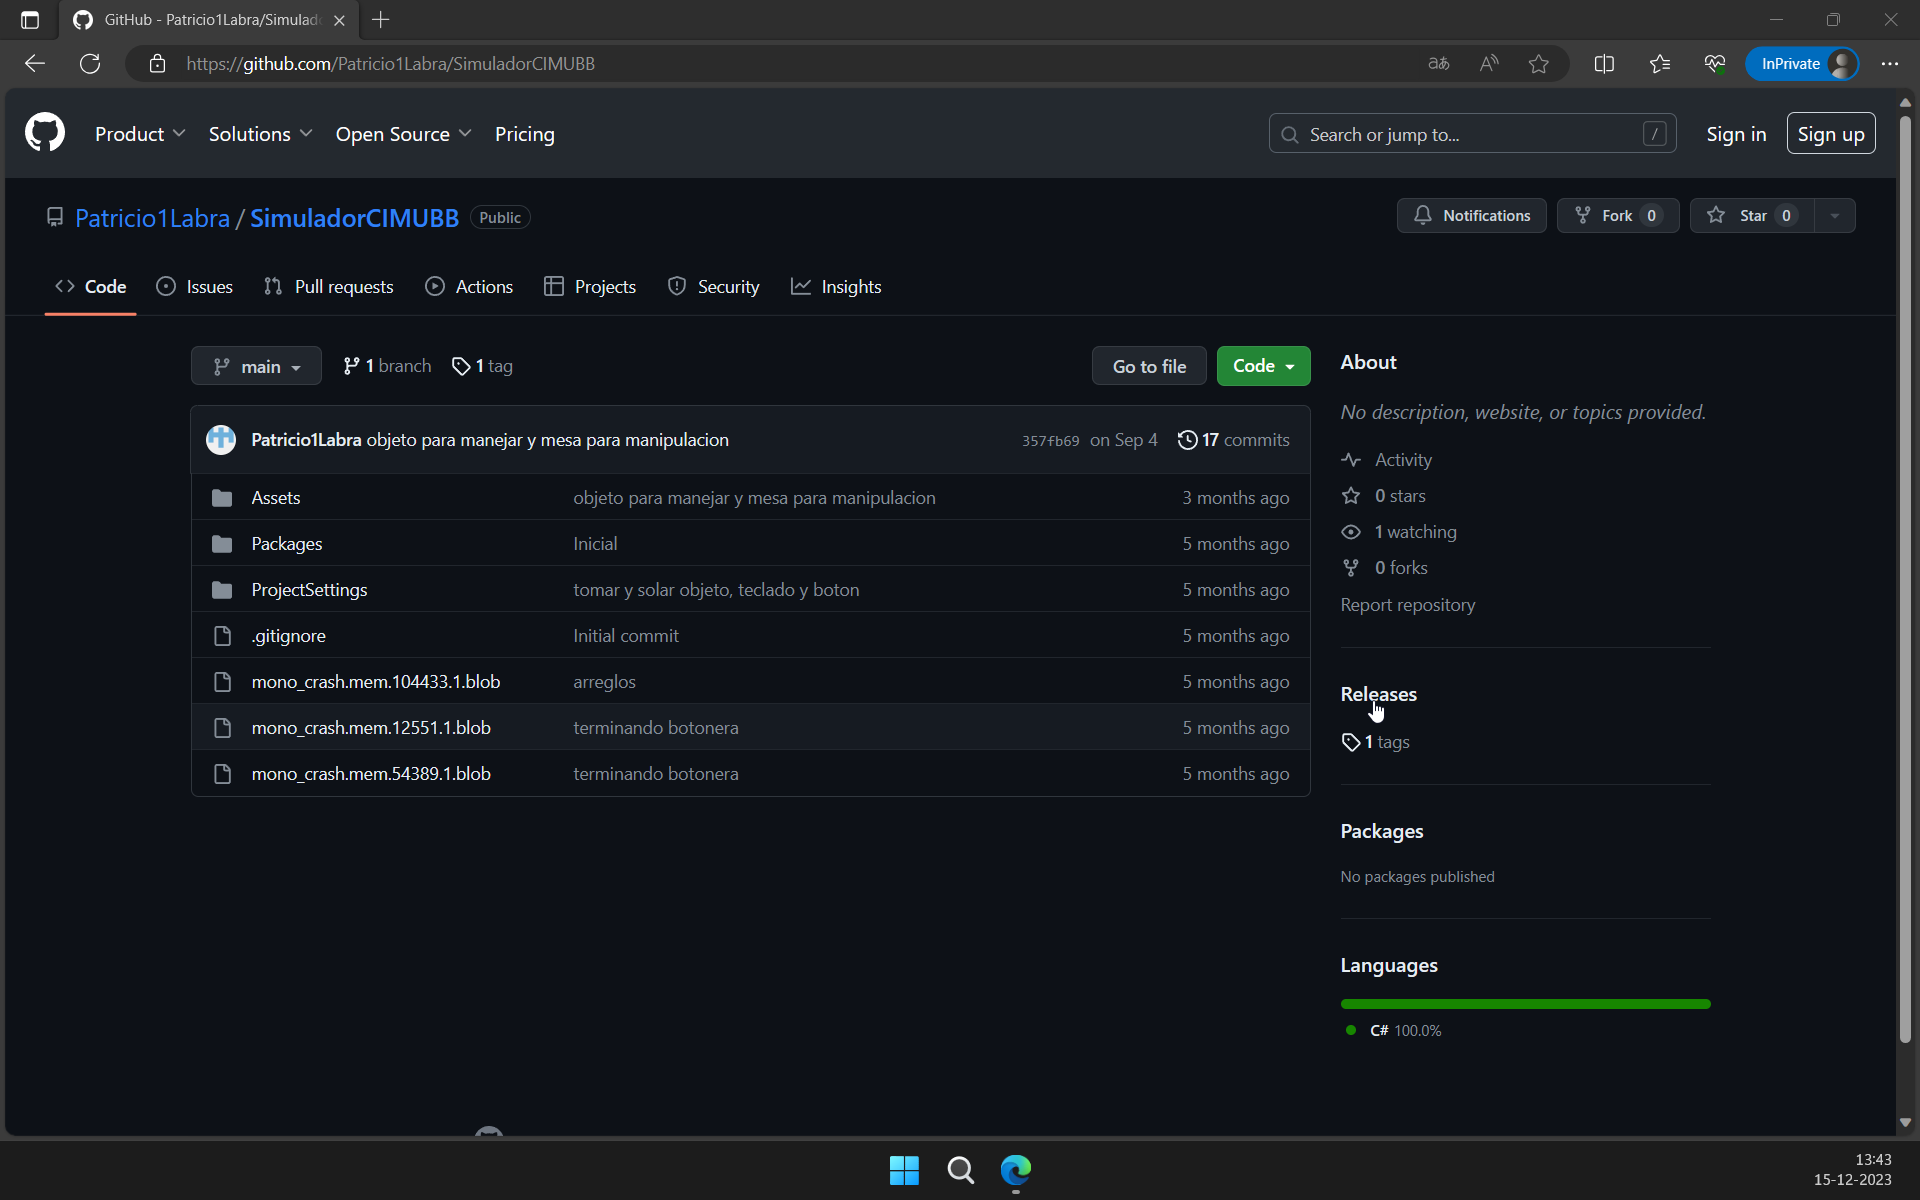
\includegraphics[width=10.5cm, height=6.5cm]{figures/TutorialWindows/tutorial (1).png}
    \caption{Parte 1 Tutorial}
    \label{fig:tuto1}
\end{figure}

\clearpage
    \item Estando en ''Releases'', buscar la ultima version, y dar click en ''Assets''.
\begin{figure}[ht]
    \centering
    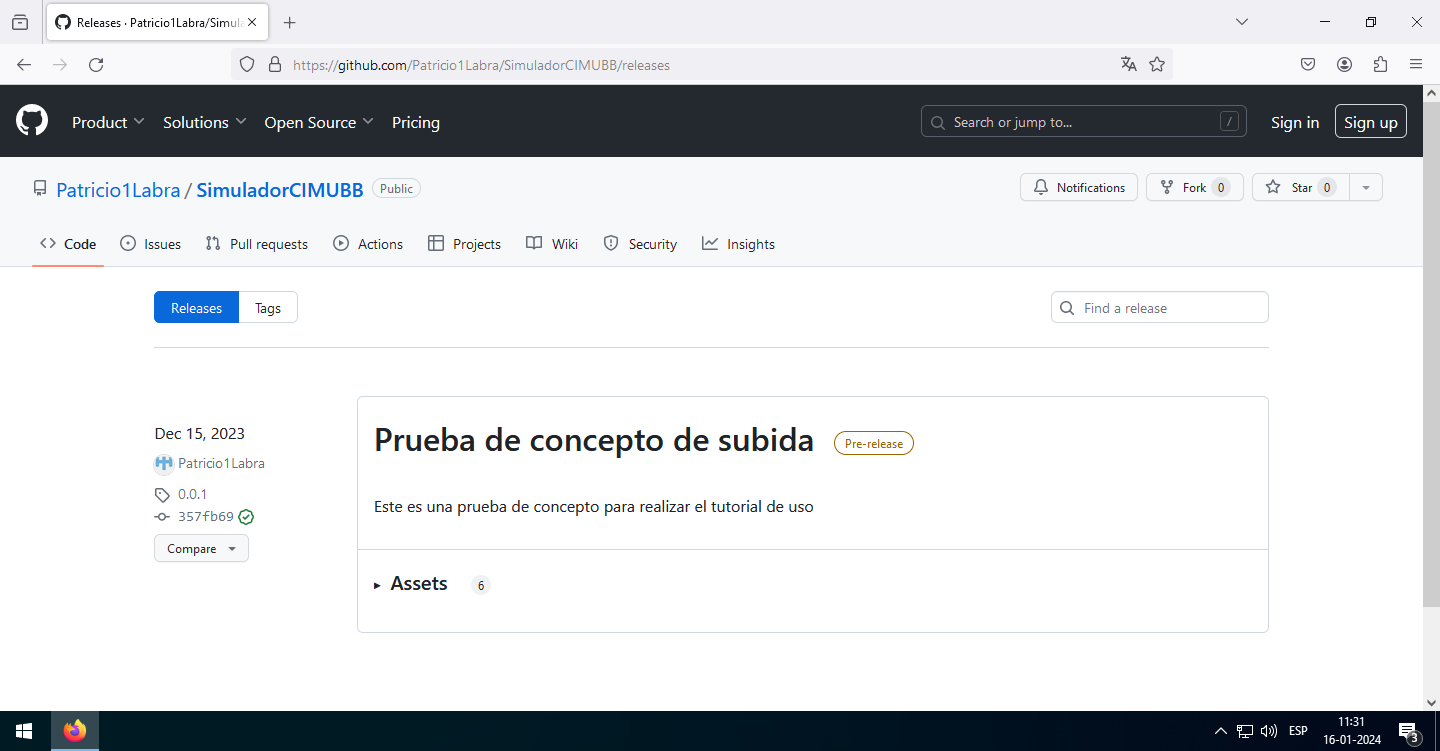
\includegraphics[width=10.5cm, height=6.5cm]{figures/TutorialWindows/tutorial (2).png}
    \caption{Parte 2 Tutorial}
    \label{fig:tuto2}
\end{figure}

    \item Elegir el archivo correspondiente al sistema.
\begin{figure}[ht]
    \centering
    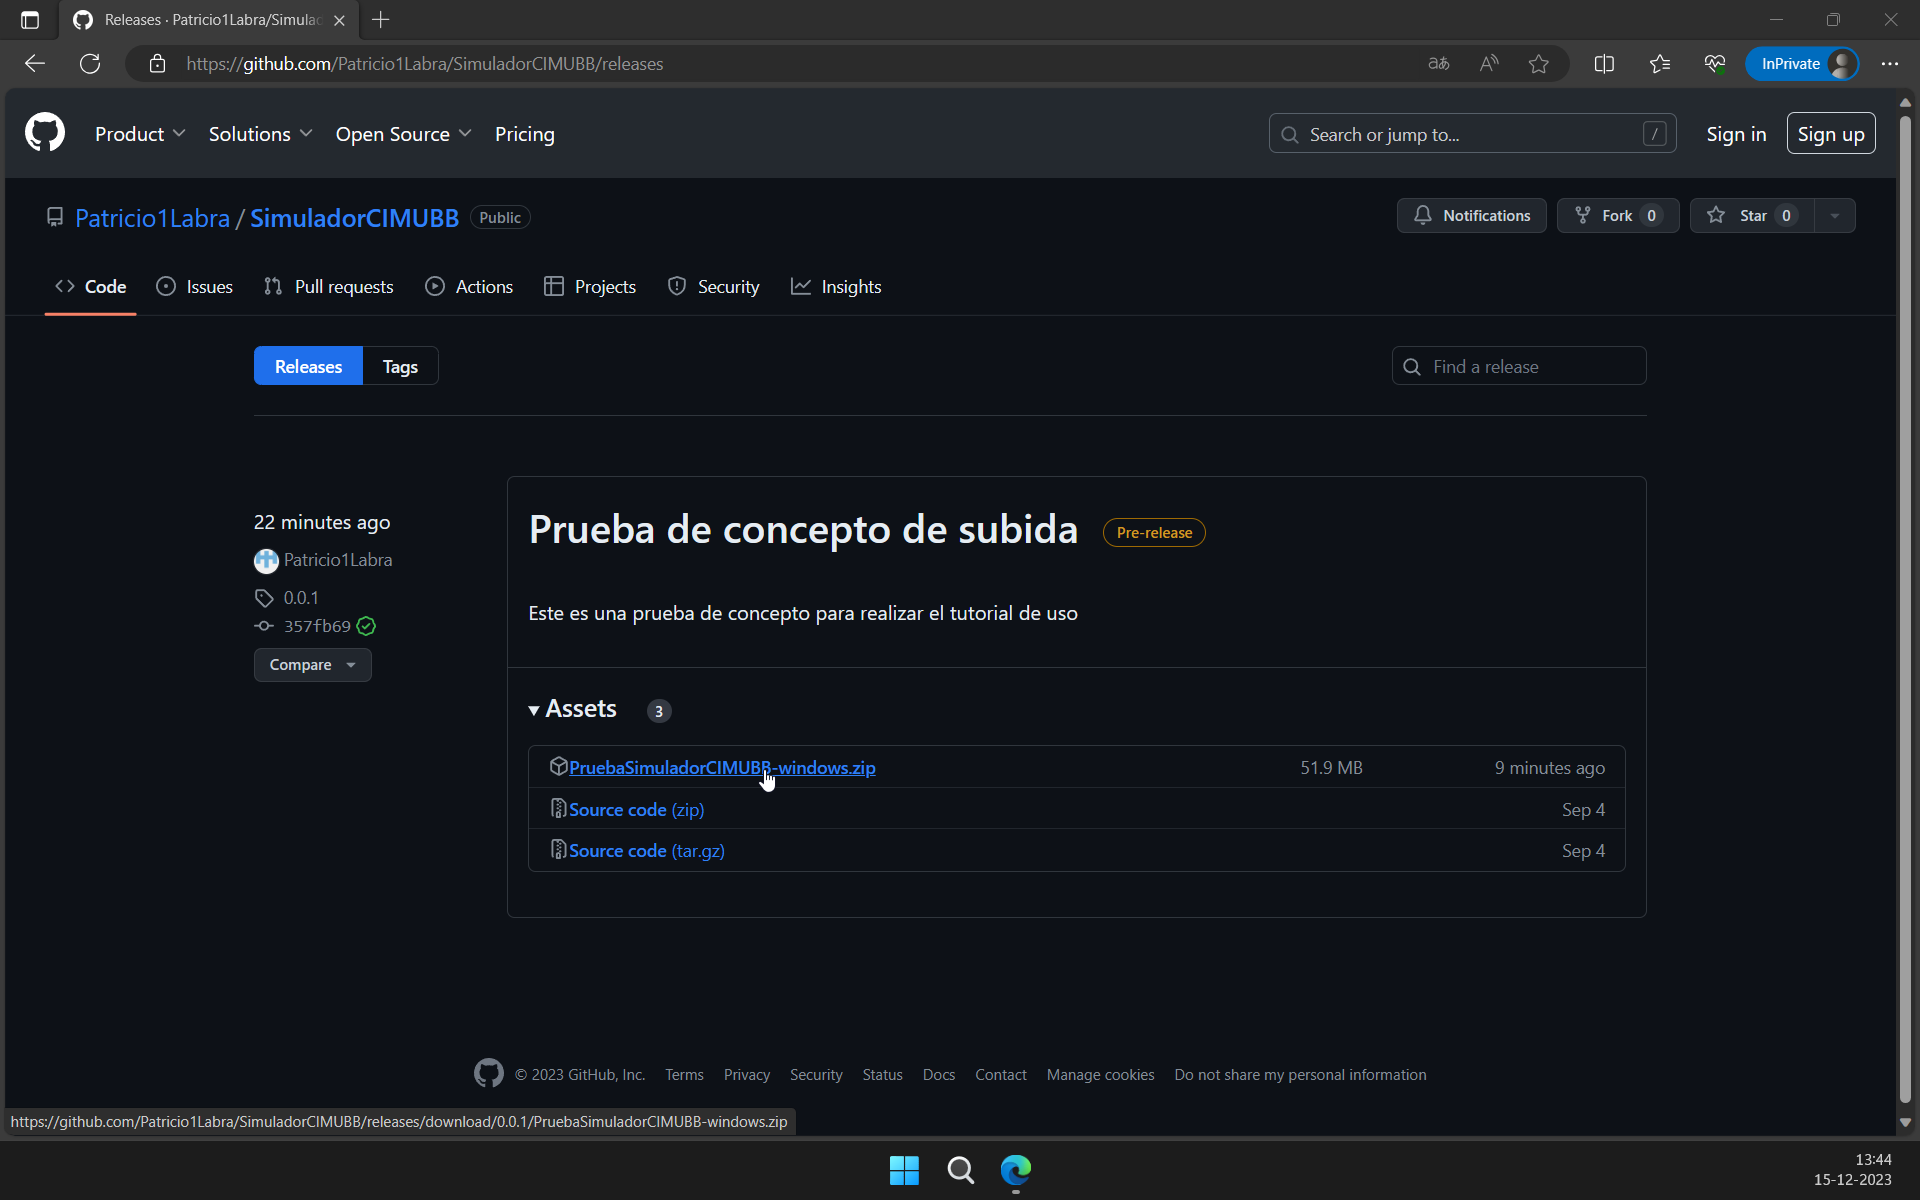
\includegraphics[width=10.5cm, height=6.5cm]{figures/TutorialWindows/tutorial (3).png}
    \caption{Parte 3 Tutorial}
    \label{fig:tuto3}
\end{figure}

\clearpage
    \item Ir a la ubicación de descarga el archivo.
\begin{figure}[ht]
    \centering
    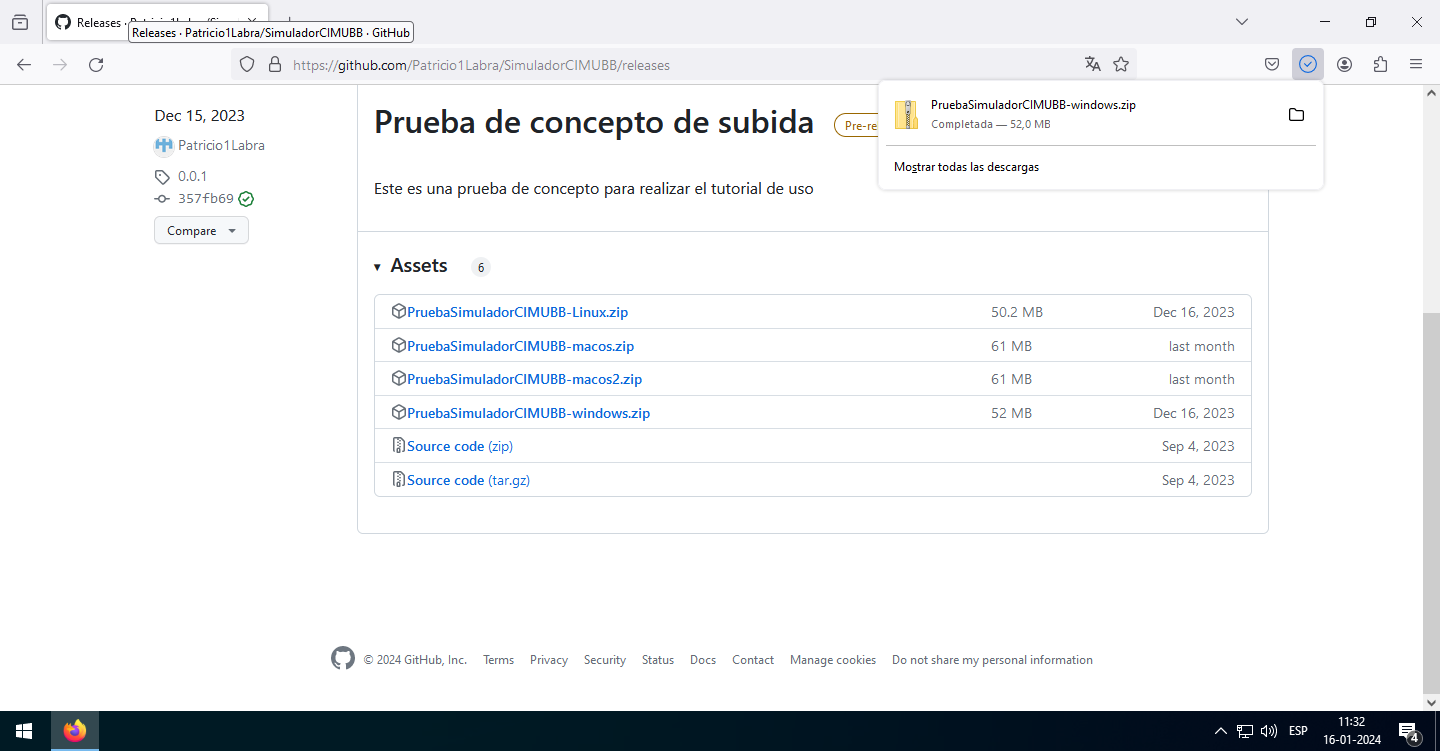
\includegraphics[width=10.5cm, height=6.5cm]{figures/TutorialWindows/tutorial (4).png}
    \caption{Parte 4 Tutorial}
    \label{fig:tuto4}
\end{figure}

    \item Estando en esta parte, se separa dependiendo el sistema a utilizar.
\begin{figure}[ht]
    \centering
    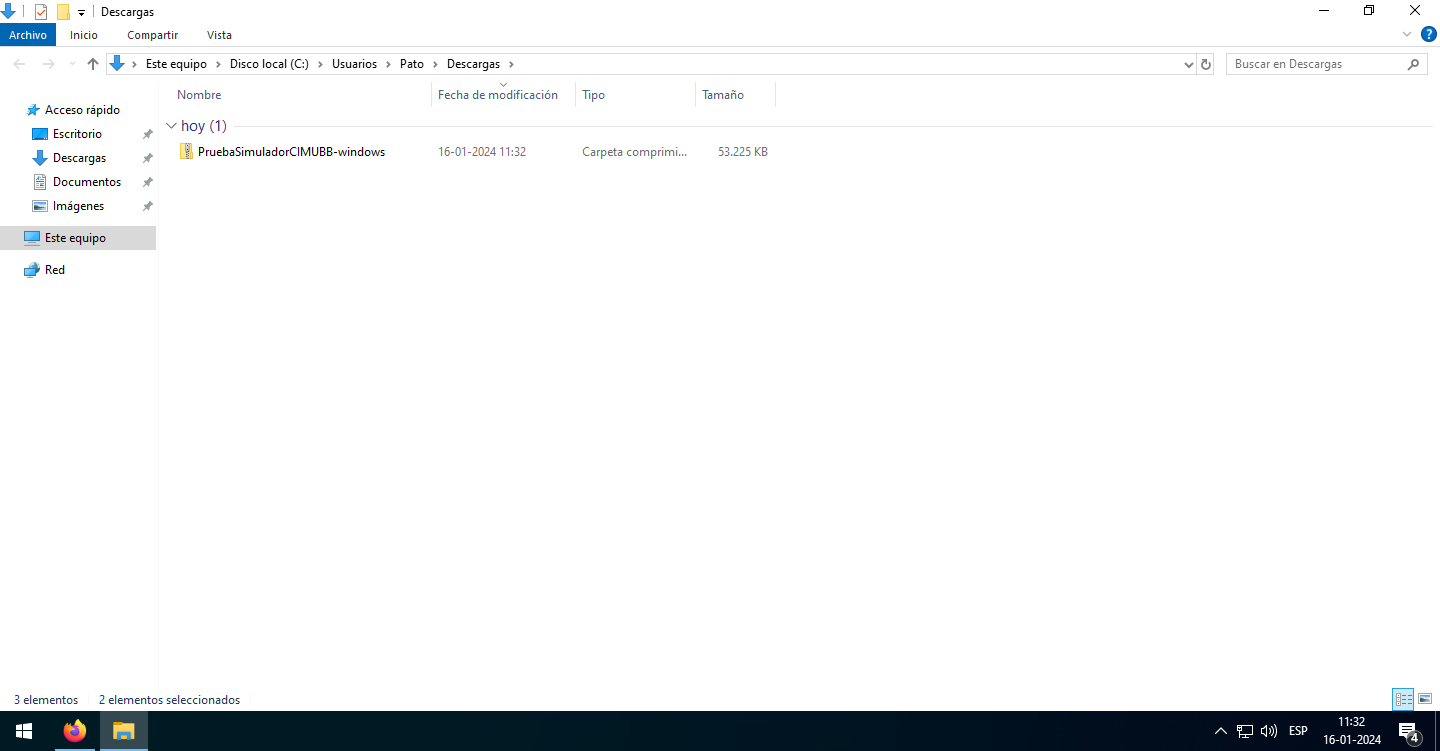
\includegraphics[width=10.5cm, height=6.5cm]{figures/TutorialWindows/tutorial (5).png}
    \caption{Parte 5 Tutorial}
    \label{fig:tuto5}
\end{figure}
\end{enumerate}
\clearpage

\subsection*{Descomprimir}

\subsubsection*{Windows}

\begin{enumerate}[label=\arabic*.-]
    \item (Opcional) Descargar e instalar WinRAR u otro programa de su preferencia para descomprimir archivos ZIP. Solo si el sistema no le permite descomprimir el archivo nativamente.
    \begin{figure}[ht]
        \centering
        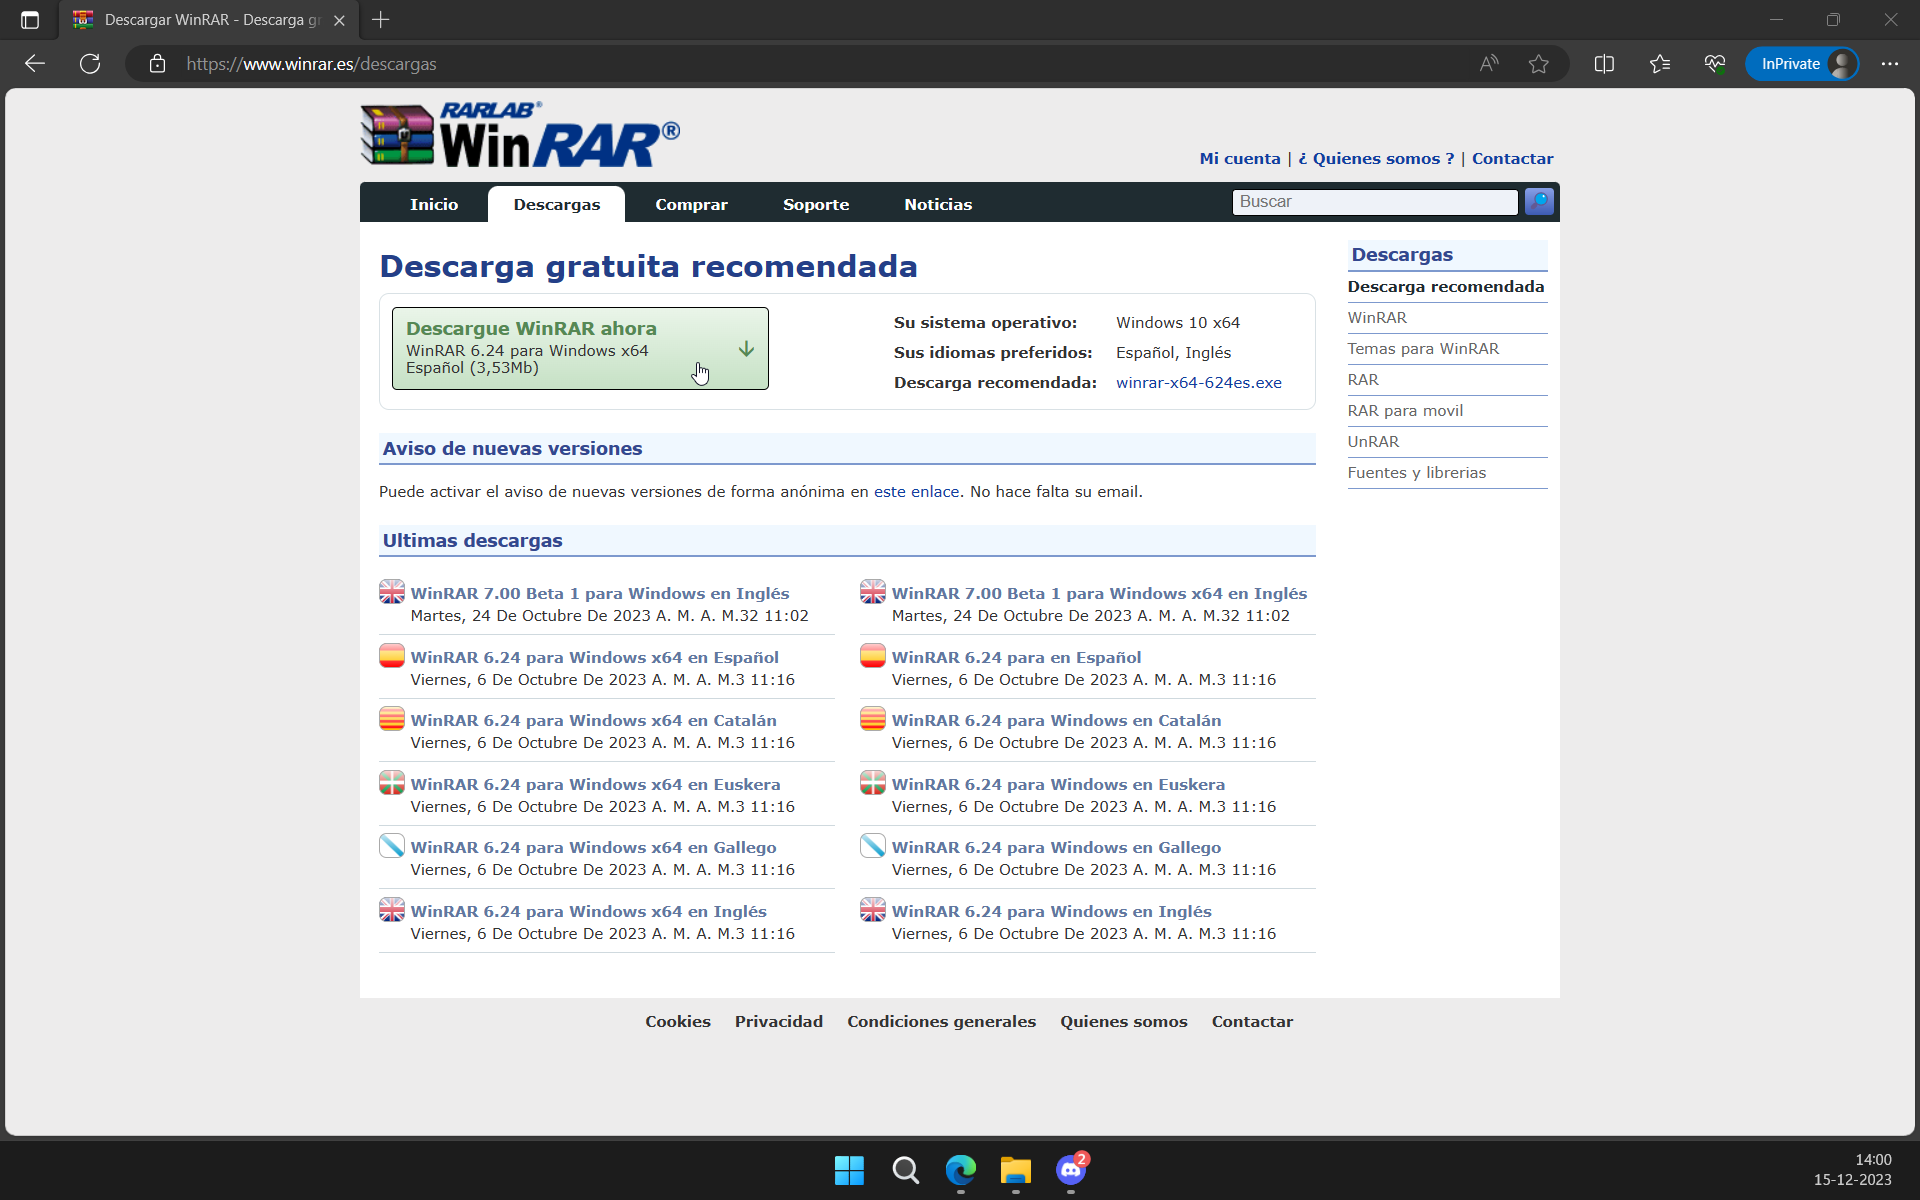
\includegraphics[width=10.5cm, height=6.5cm]{figures/TutorialWindows/winrar.png}
        \caption{Página de descarga WinRAR}
        \label{fig:winrar}
    \end{figure}

    \item Seleccionando el archivo descargado, elegir la opción ''Extraer todo''.
\begin{figure}[ht]
    \centering
    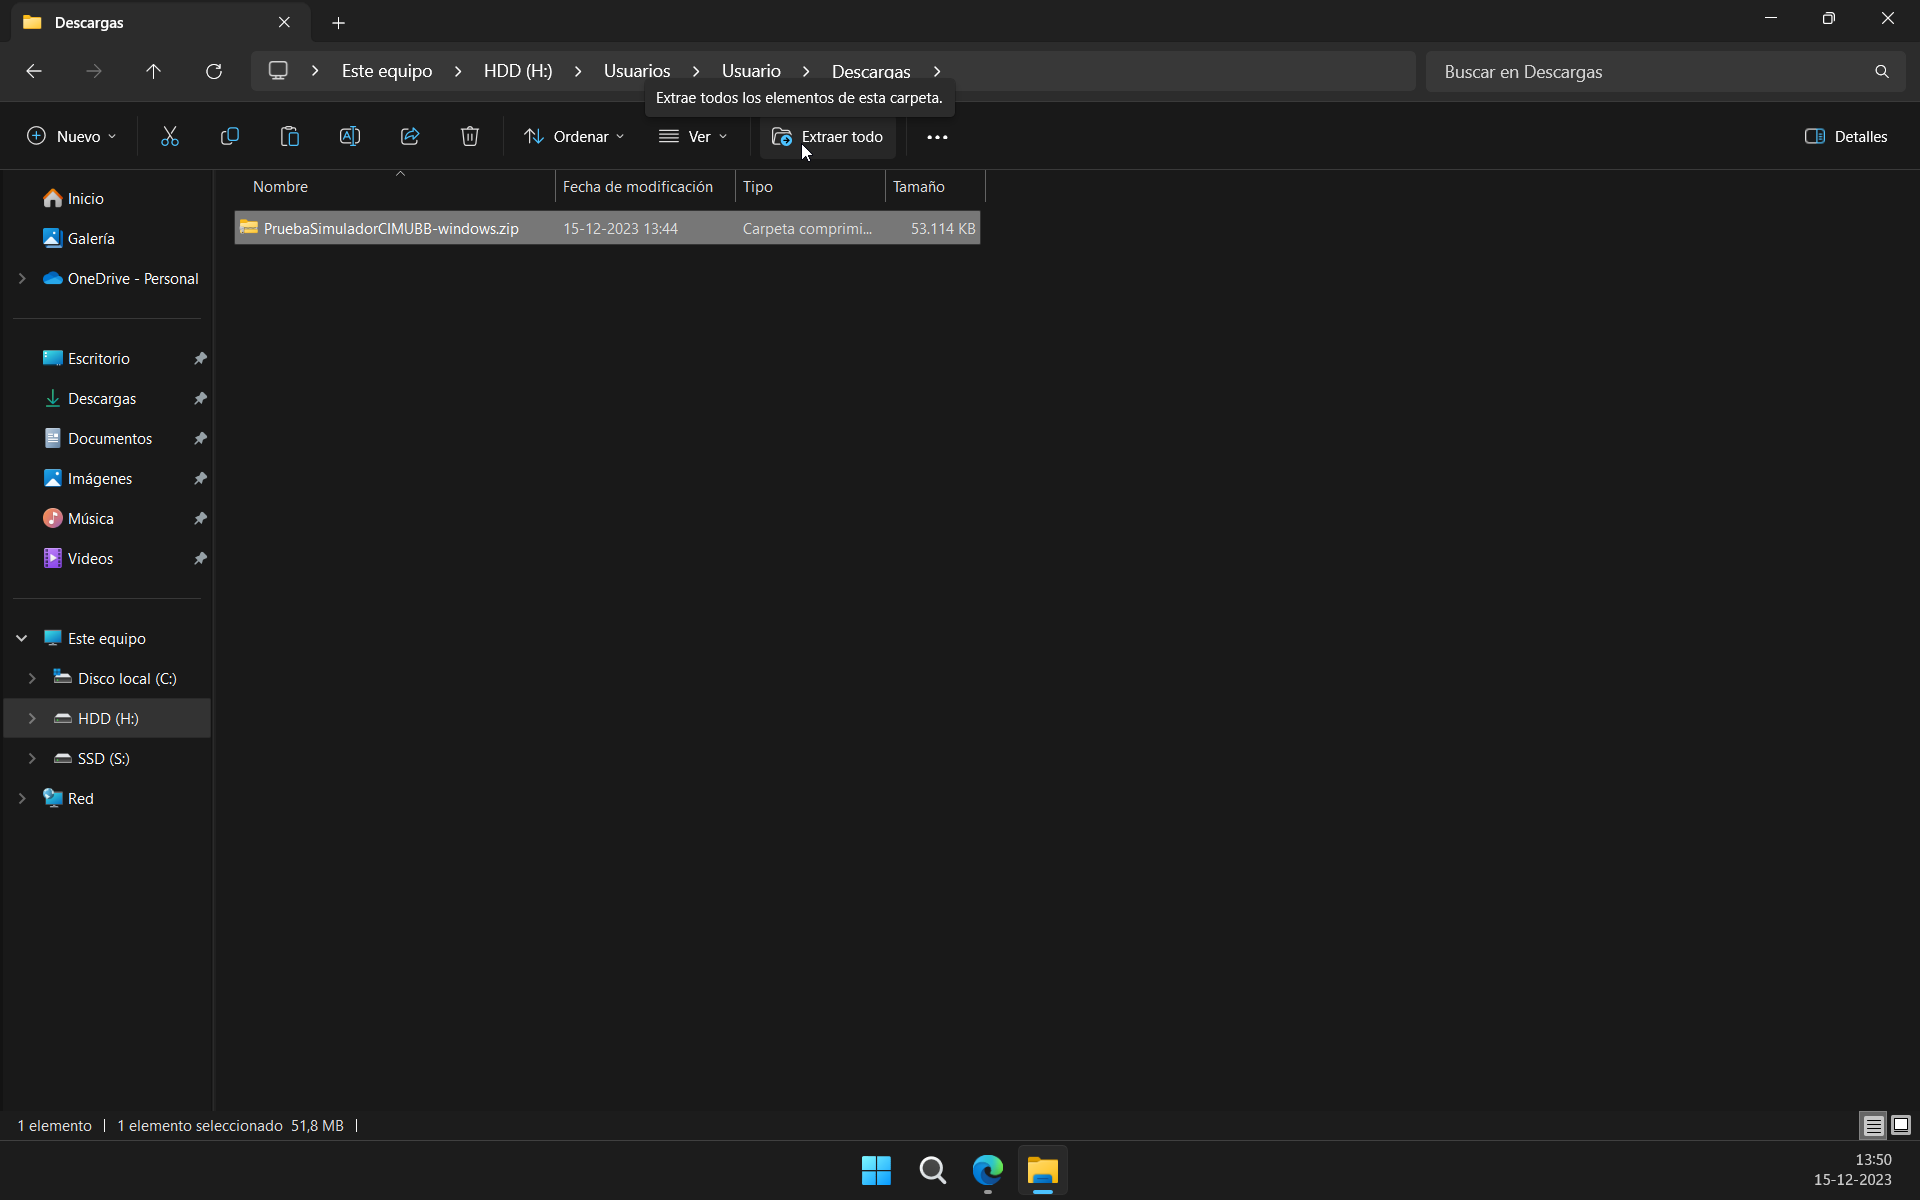
\includegraphics[width=10.5cm, height=6.5cm]{figures/TutorialWindows/tutorial (6).png}
    \caption{Parte 1 Tutorial Windows}
    \label{fig:tutowin1}
\end{figure}
\clearpage

    \item Darle al botón ''Extraer''.
\begin{figure}[ht]
    \centering
    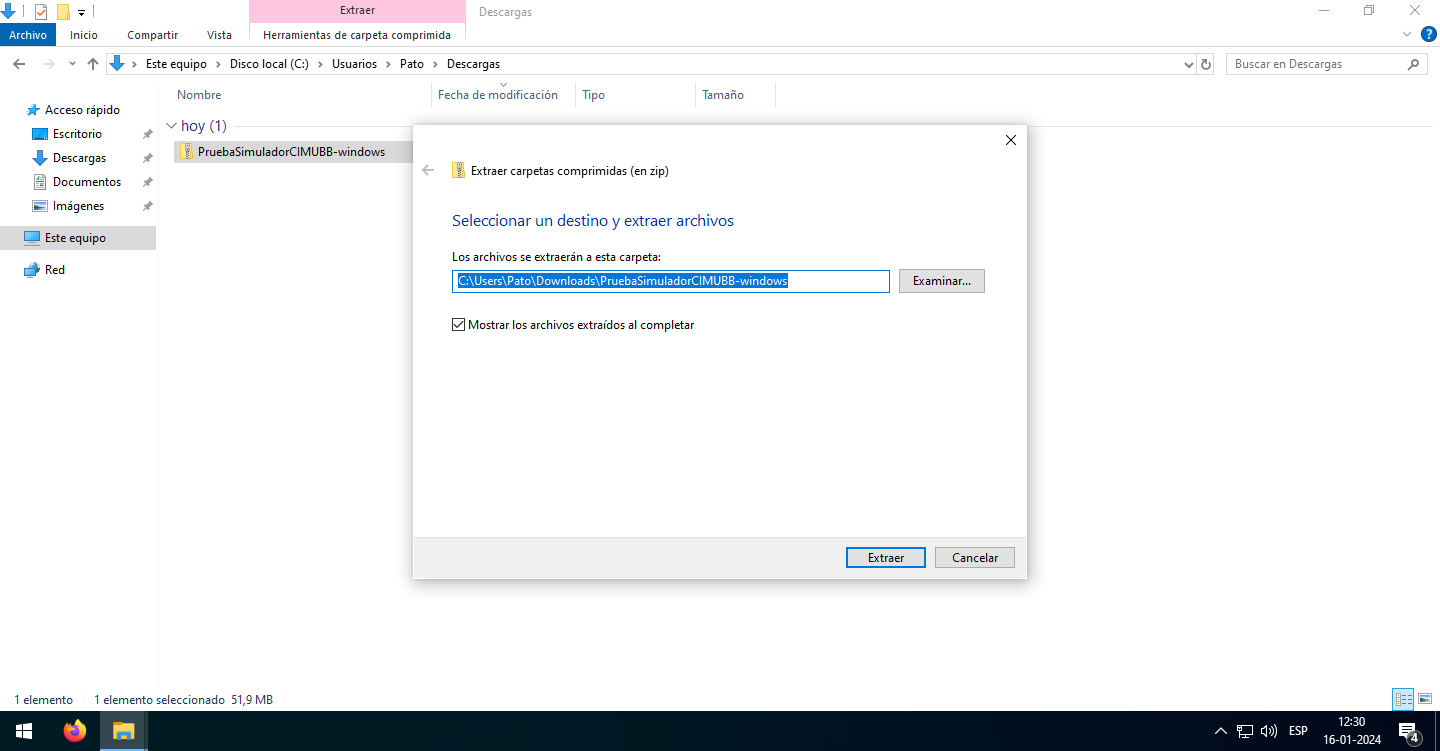
\includegraphics[width=10.5cm]{figures/TutorialWindows/tutorial (7).png}
    \caption{Parte 2 Tutorial Windows}
    \label{fig:tutowin2}
\end{figure}

    \item Abrir la nueva carpeta donde se extrajo el programa.
\begin{figure}[ht]
    \centering
    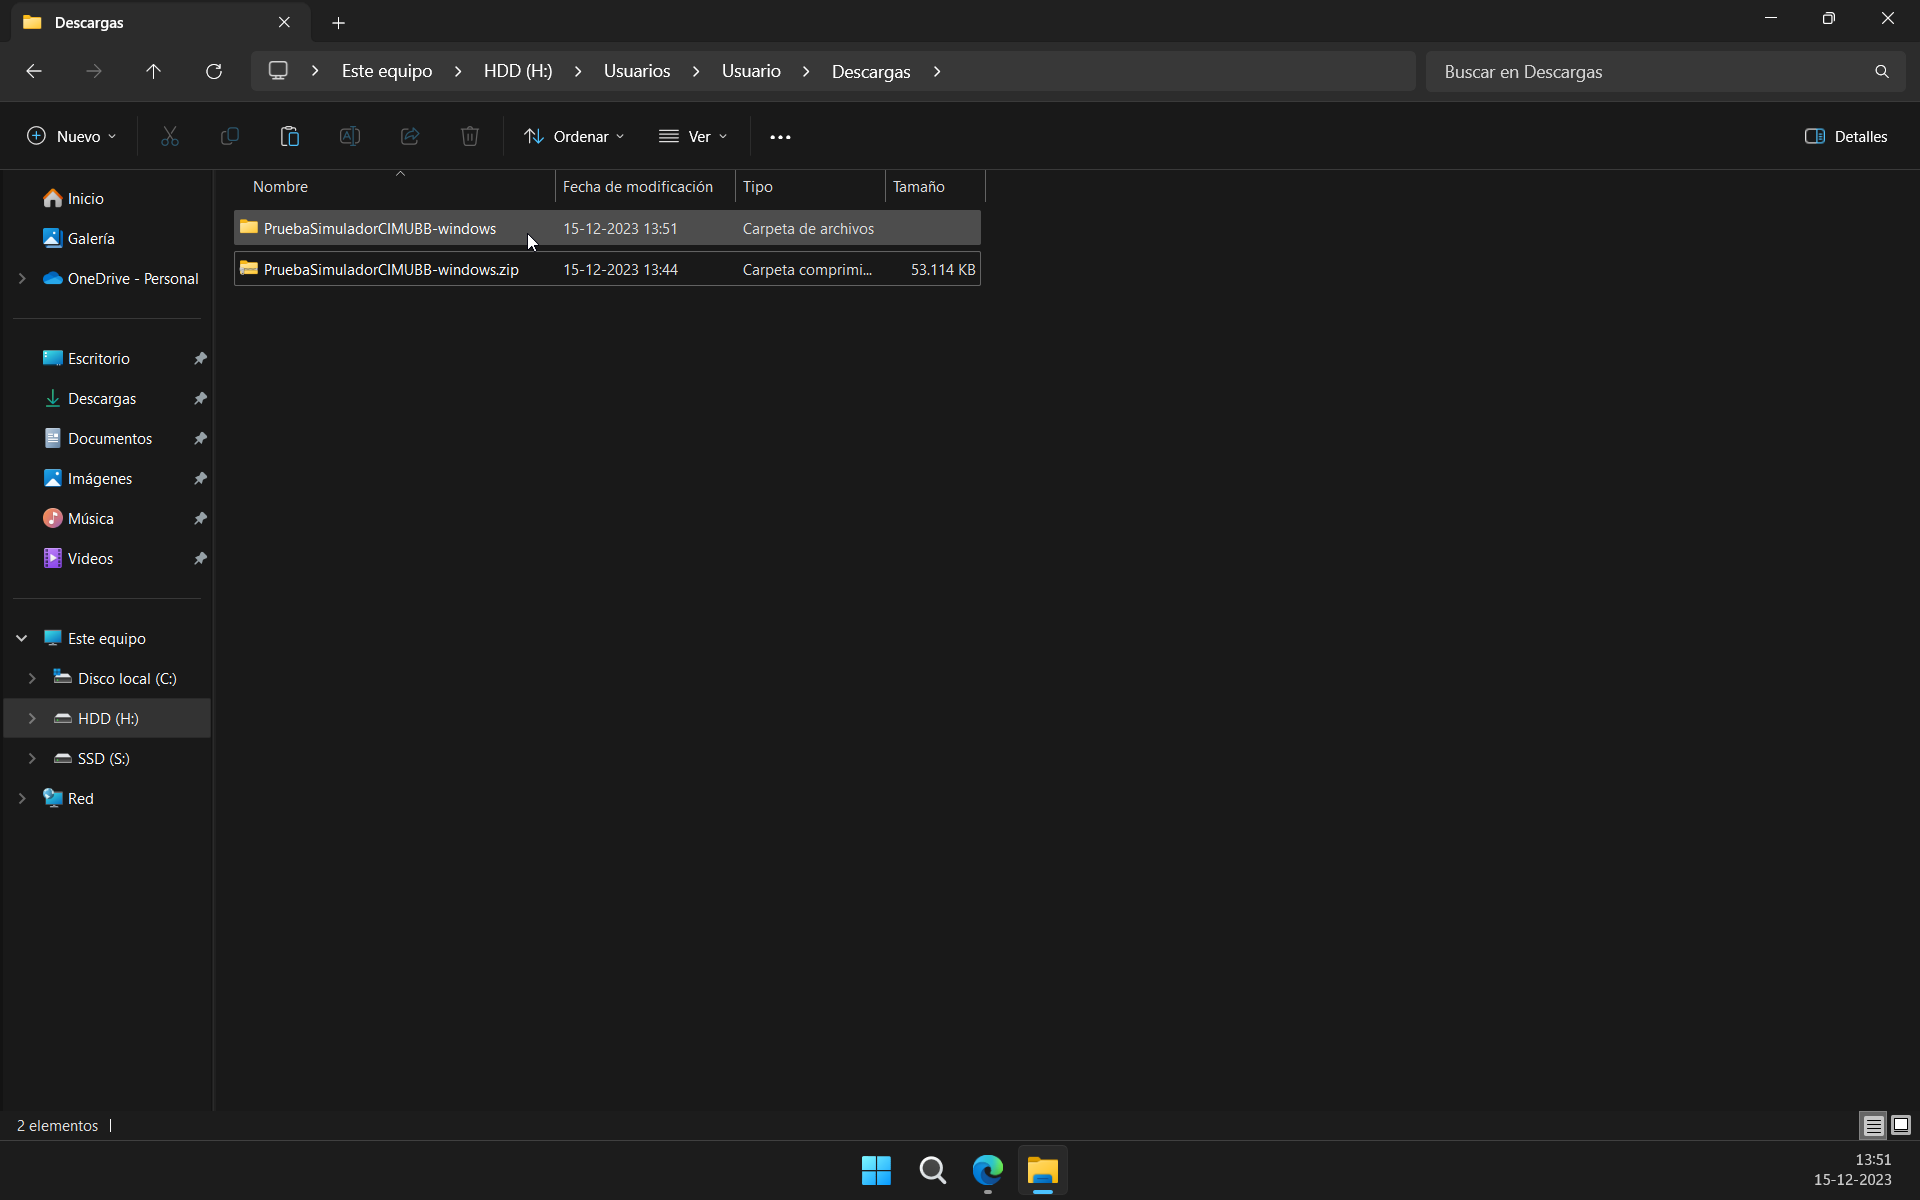
\includegraphics[width=10.5cm]{figures/TutorialWindows/tutorial (8).png}
    \caption{Parte 3 Tutorial Windows}
    \label{fig:tutowin3}
\end{figure}
\clearpage

    \item Ejecutar el archivo ''Simulador.exe''.
\begin{figure}[ht]
    \centering
    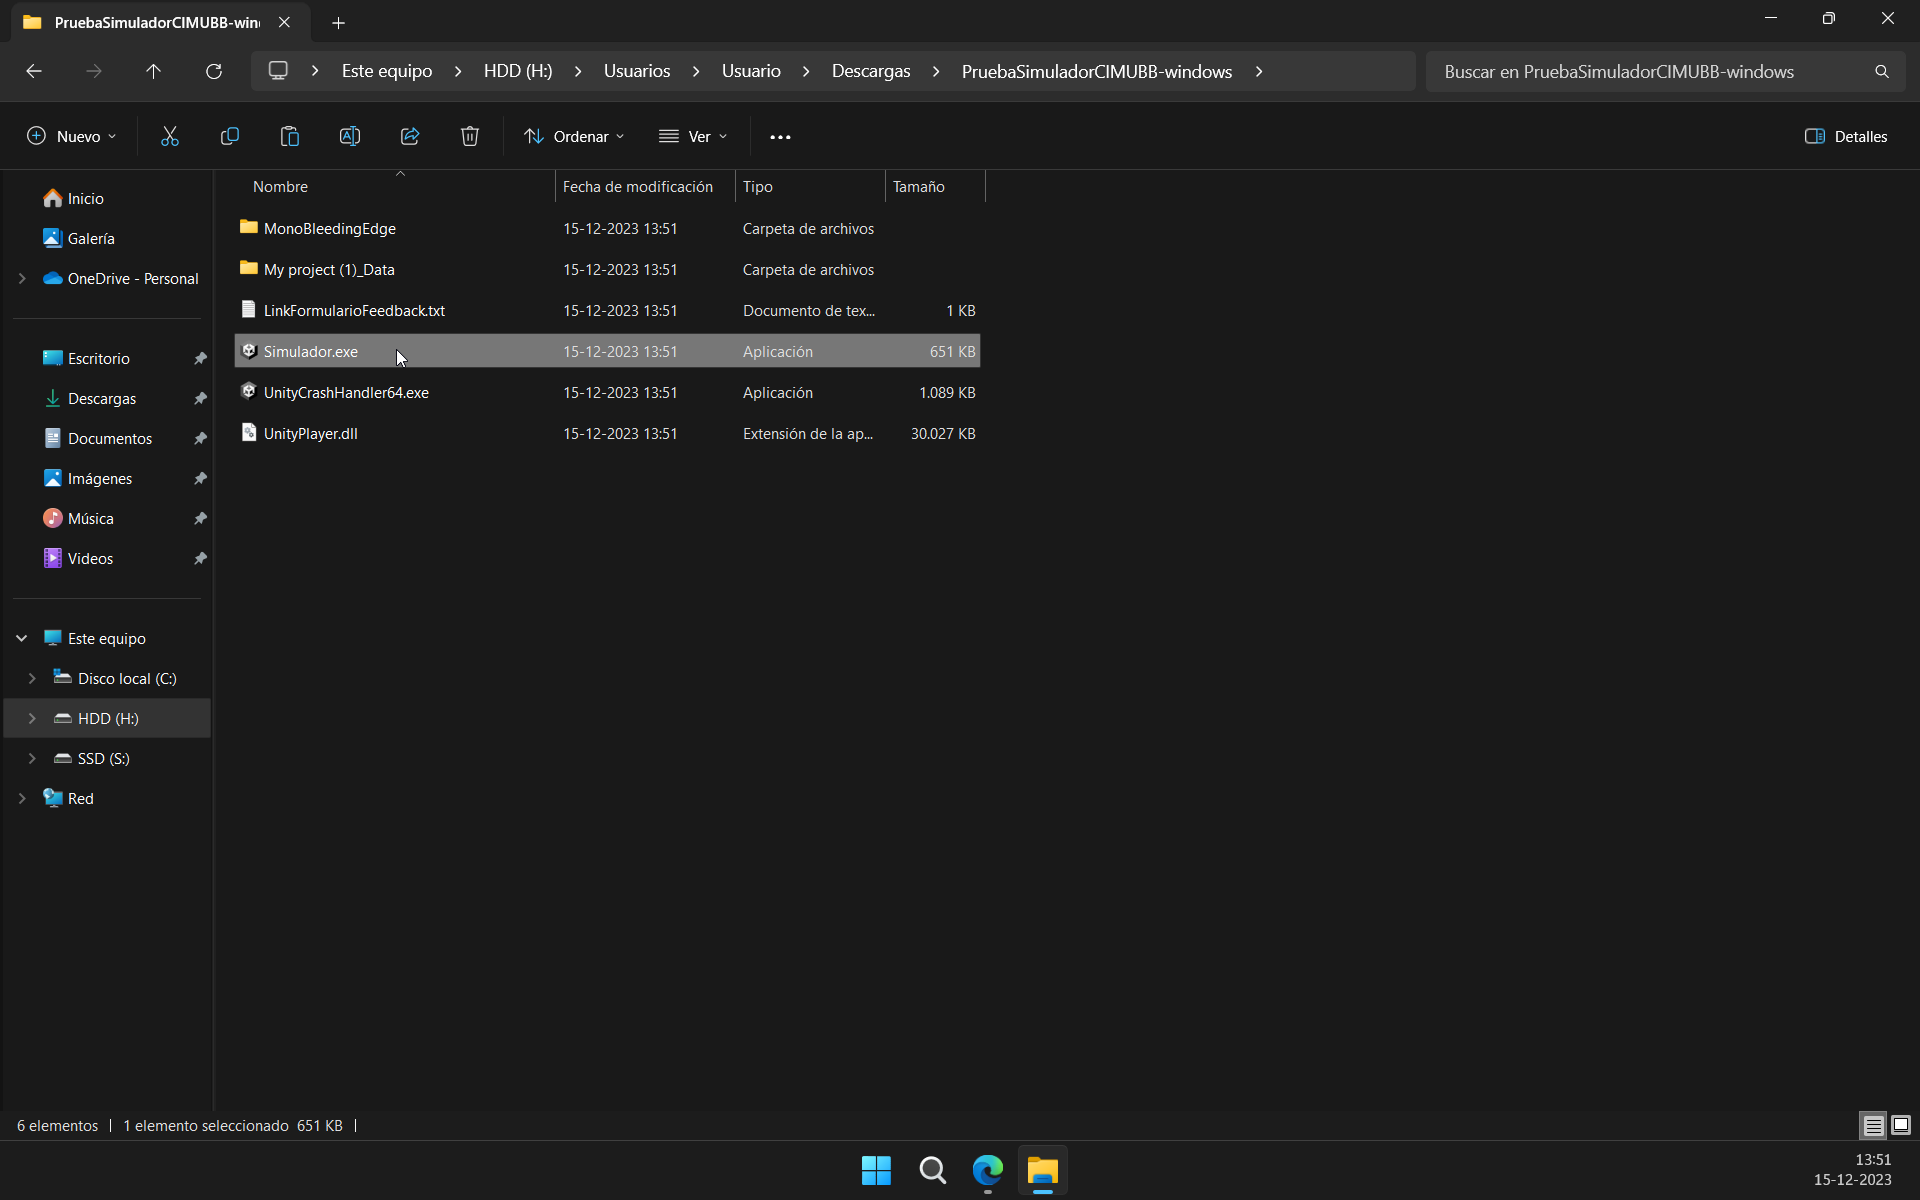
\includegraphics[width=10.5cm]{figures/TutorialWindows/tutorial (9).png}
    \caption{Parte 4 Tutorial Windows}
    \label{fig:tutowin4}
\end{figure}

    \item Algunas veces, Windows dará una advertencia, darle a ''Mas información''
\begin{figure}[ht]
    \centering
    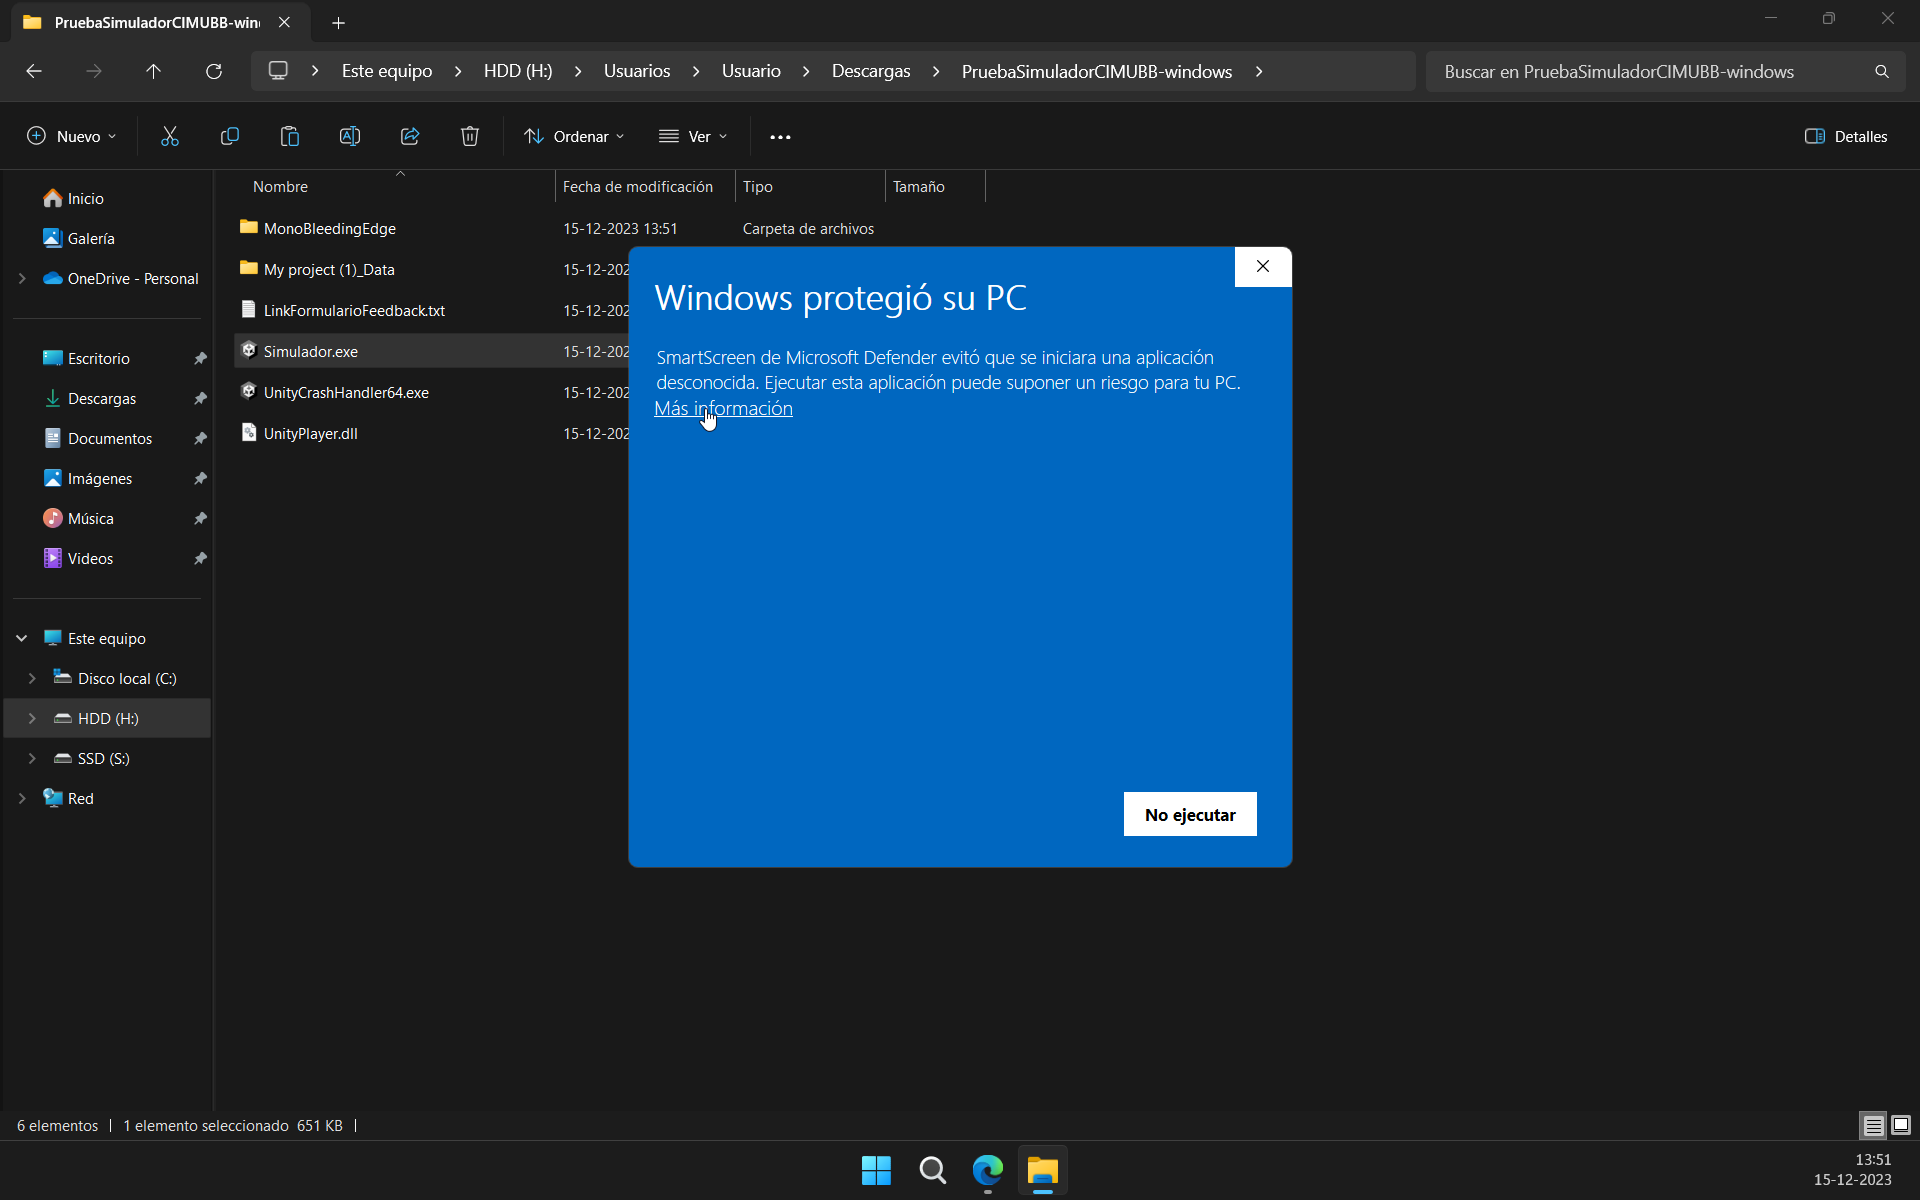
\includegraphics[width=10.5cm]{figures/TutorialWindows/tutorial (10).png}
    \caption{Parte 5 Tutorial Windows}
    \label{fig:tutowin5}
\end{figure}
\clearpage

    \item Dar al botón ''Ejecutar de todas formas''.
\begin{figure}[ht]
    \centering
    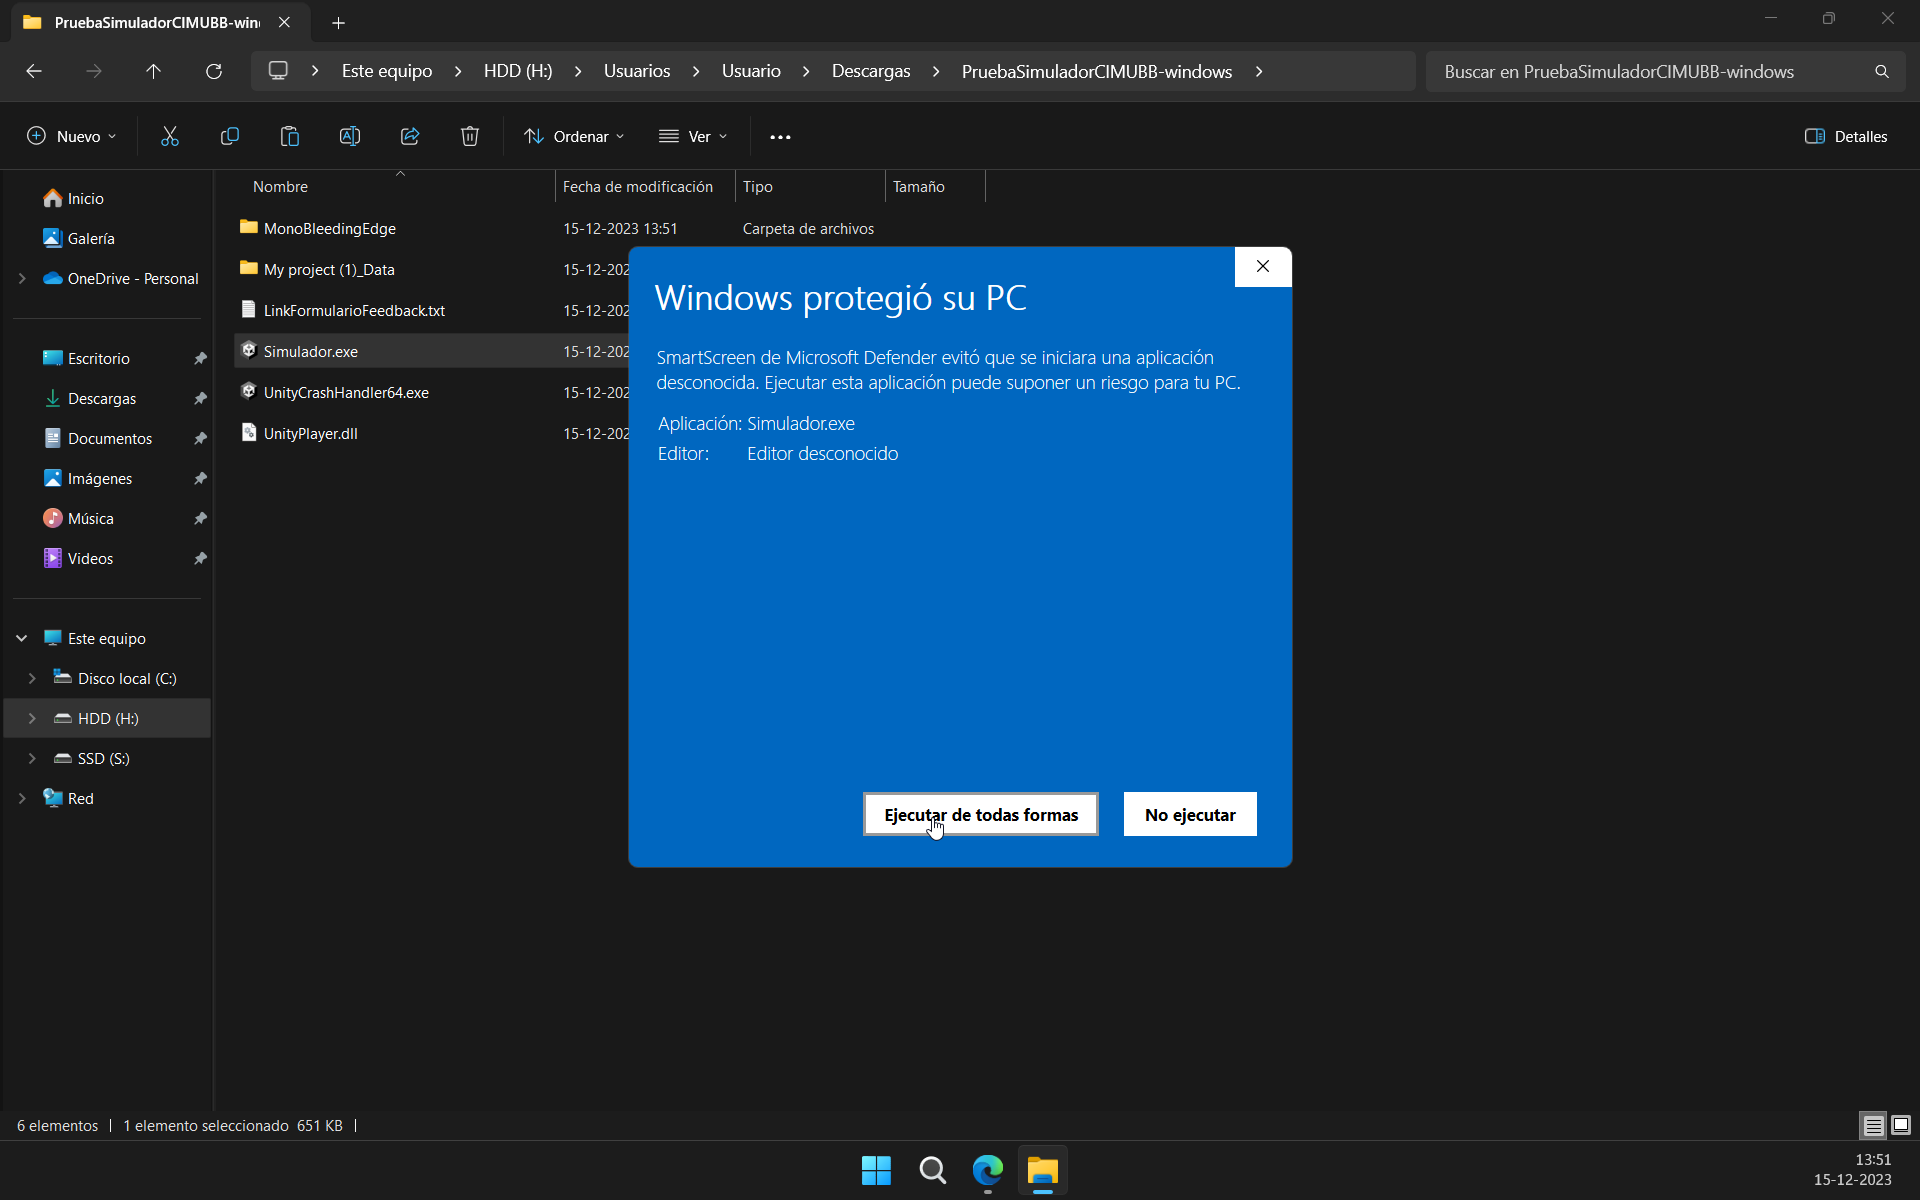
\includegraphics[width=10.5cm]{figures/TutorialWindows/tutorial (11).png}
    \caption{Parte 6 Tutorial Windows}
    \label{fig:tutowin6}
\end{figure}

    \item La aplicación iniciara.
\begin{figure}[ht]
    \centering
    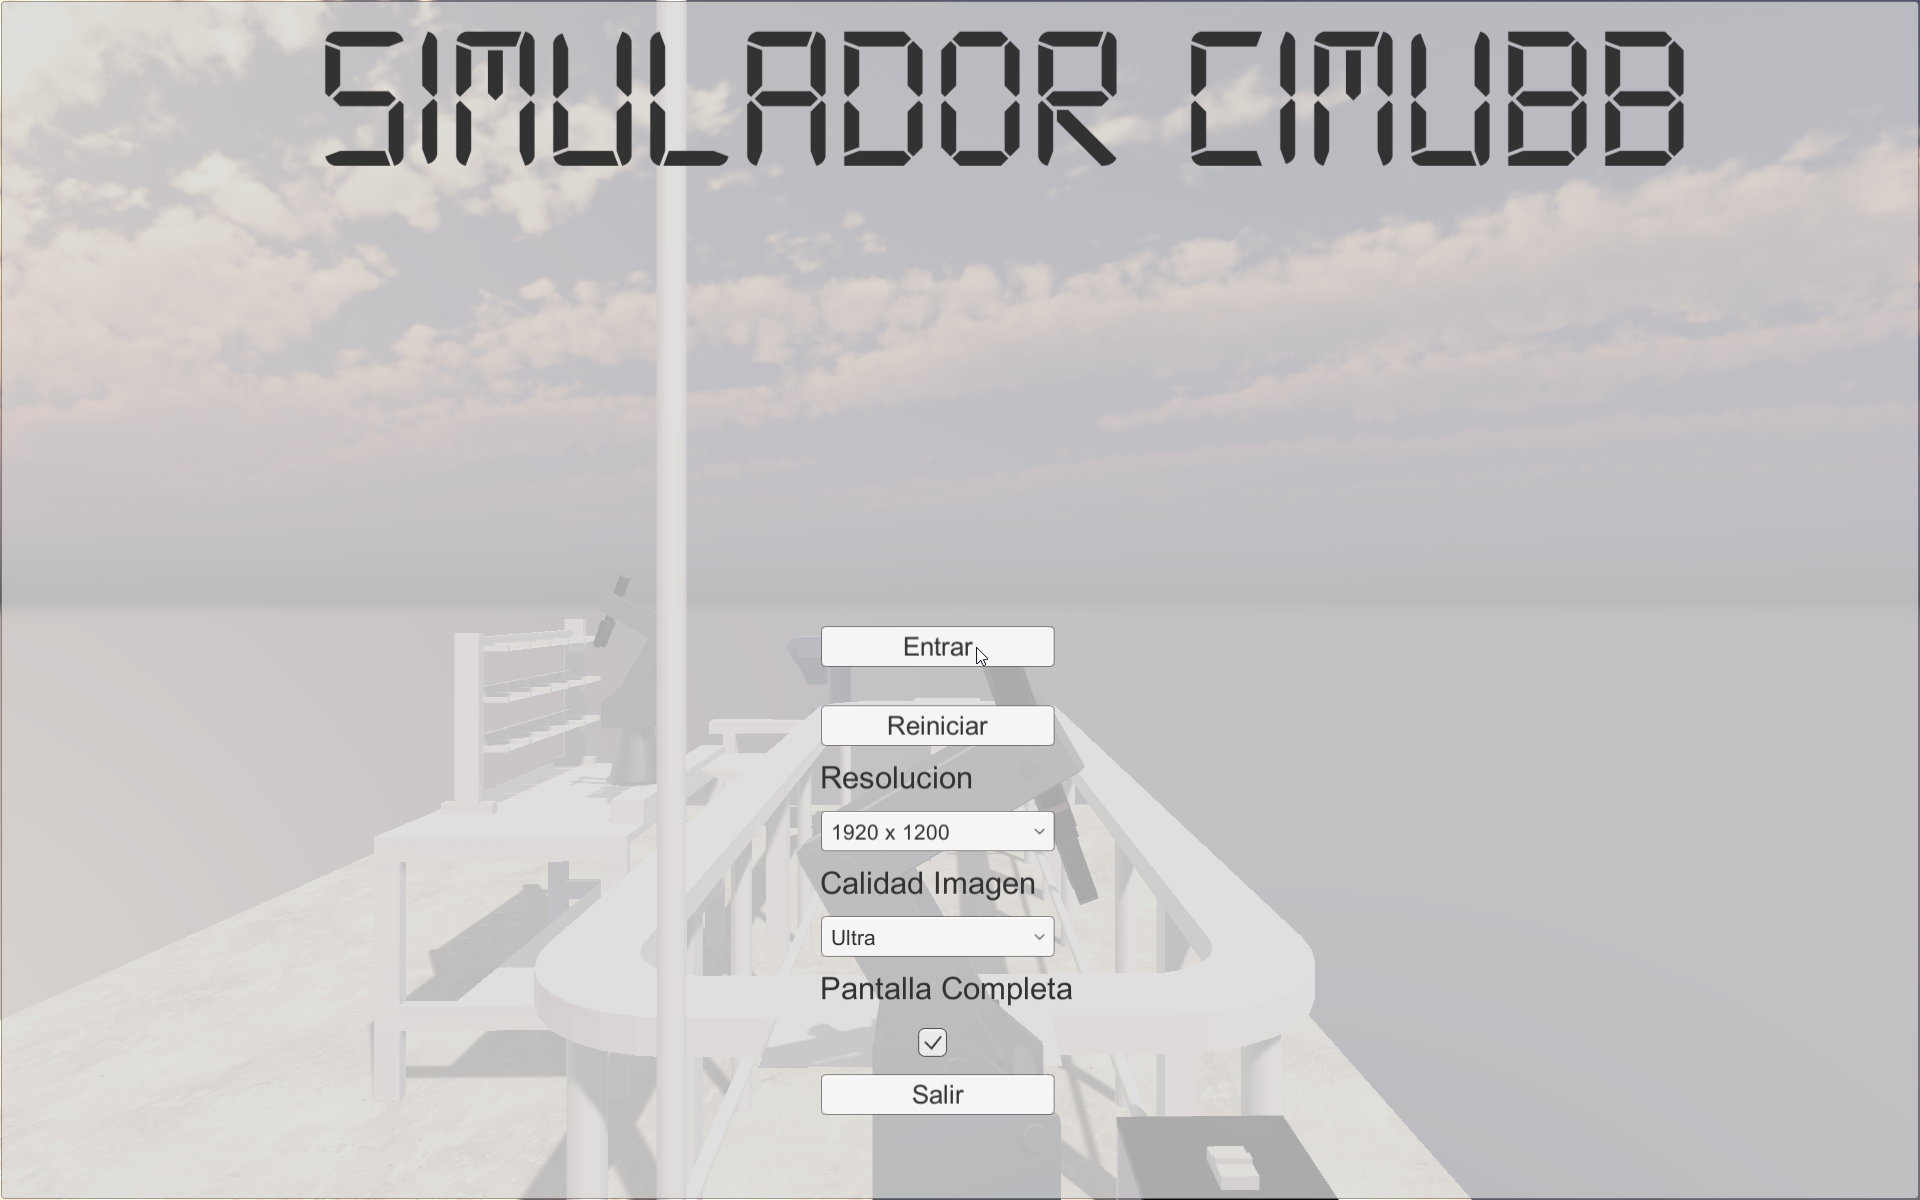
\includegraphics[width=10.5cm]{figures/TutorialWindows/tutorial (12).png}
    \caption{Parte 7 Tutorial Windows}
    \label{fig:tutowin7}
\end{figure}
\end{enumerate}
\clearpage

\subsubsection*{Linux}

\begin{enumerate}[label=\arabic*.-]
    \item Estando en la carpeta de descarga, se tienen dos opciones para descomprimir.
\begin{figure}[ht]
    \centering
    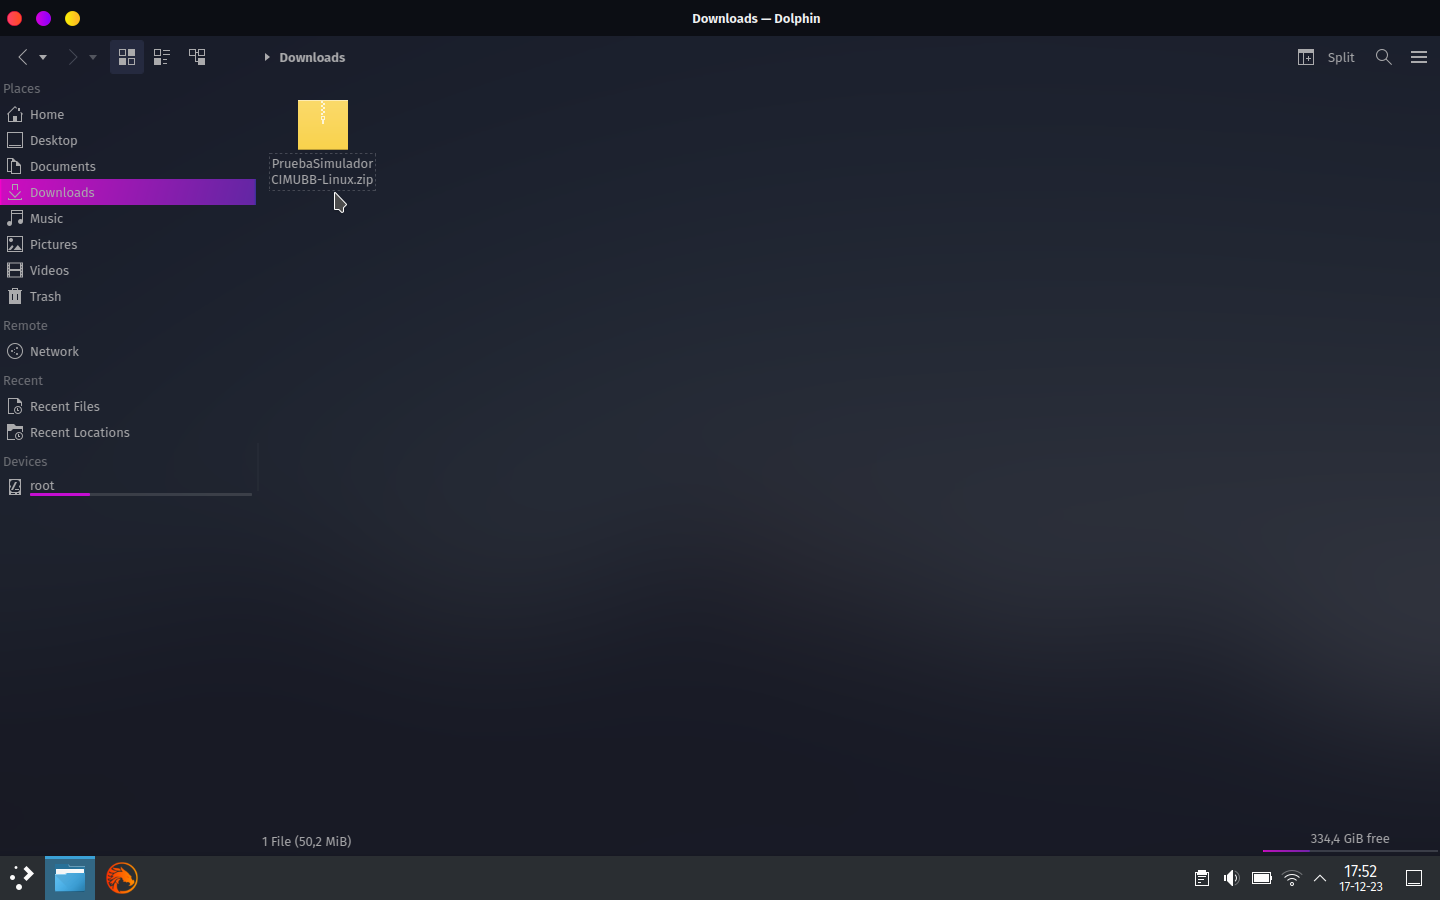
\includegraphics[width=10.5cm]{figures/TutorialLinux/tutoriallinux (1).png}
    \caption{Parte 1 Tutorial Linux}
    \label{fig:tutolinux1}
\end{figure}

    \item Al hacer click derecho, se da la opción de extraer.
\begin{figure}[ht]
    \centering
    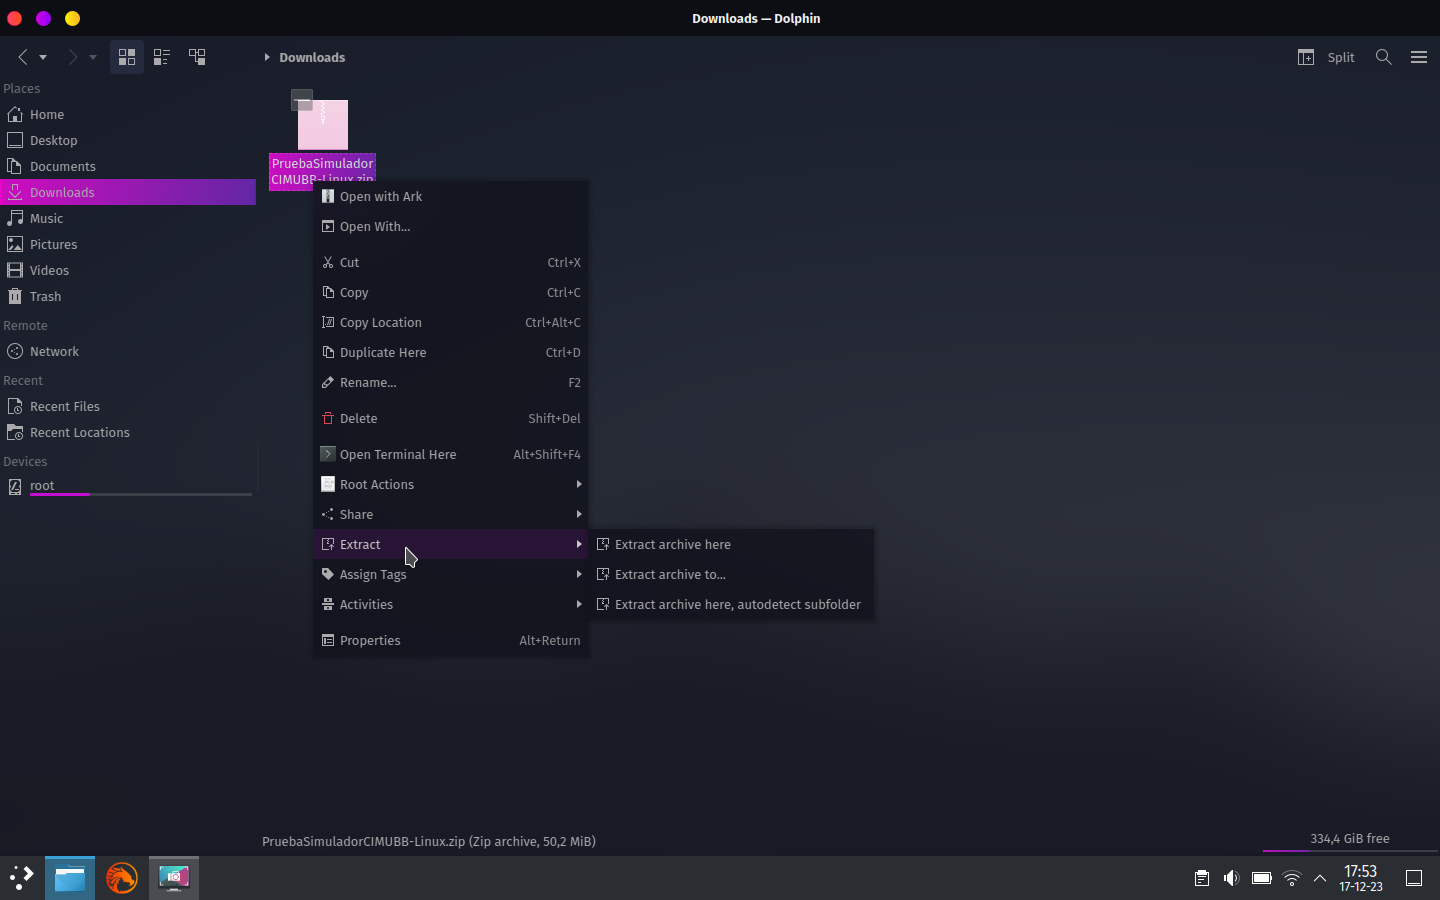
\includegraphics[width=10.5cm]{figures/TutorialLinux/tutoriallinux (2).png}
    \caption{Parte 2.1 Tutorial Linux}
    \label{fig:tutolinux2}
\end{figure}
\clearpage

    \item Si la distribución de Linux no posee esa opción, hacer click derecho para abrir la terminal en la carpeta.
\begin{figure}[ht]
    \centering
    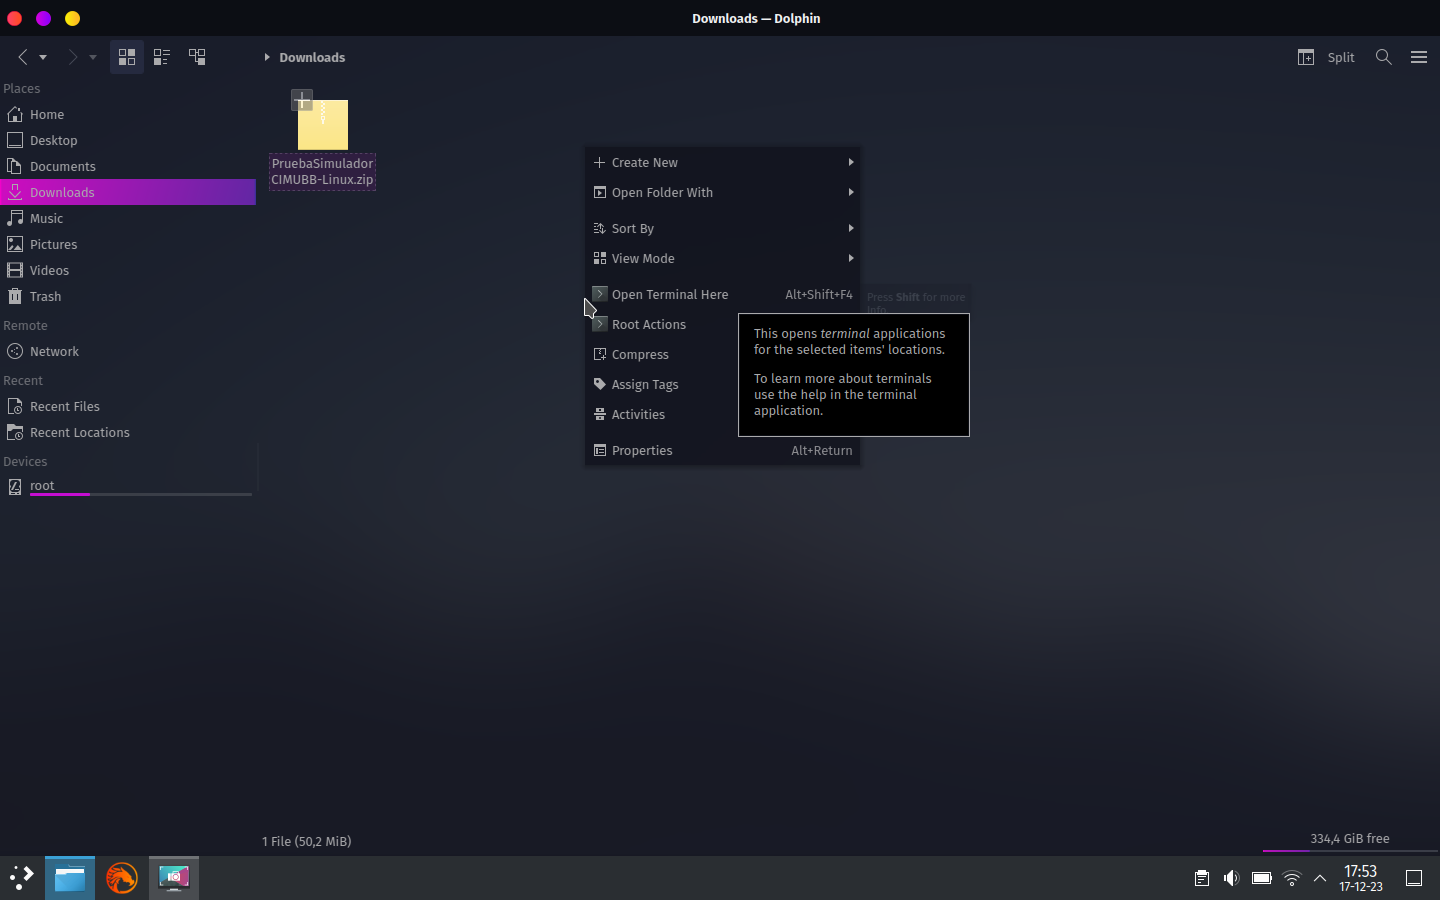
\includegraphics[width=10.5cm]{figures/TutorialLinux/tutoriallinux (3).png}
    \caption{Parte 2.2.1 Tutorial Linux}
    \label{fig:tutolinux3}
\end{figure}

    \item Verificar que ''unzip'' esta instalado usando la opción ''unzip -v'' (Si no se encuentra disponible, buscar el método de instalación para la distribución Linux correspondiente).
\begin{figure}[ht]
    \centering
    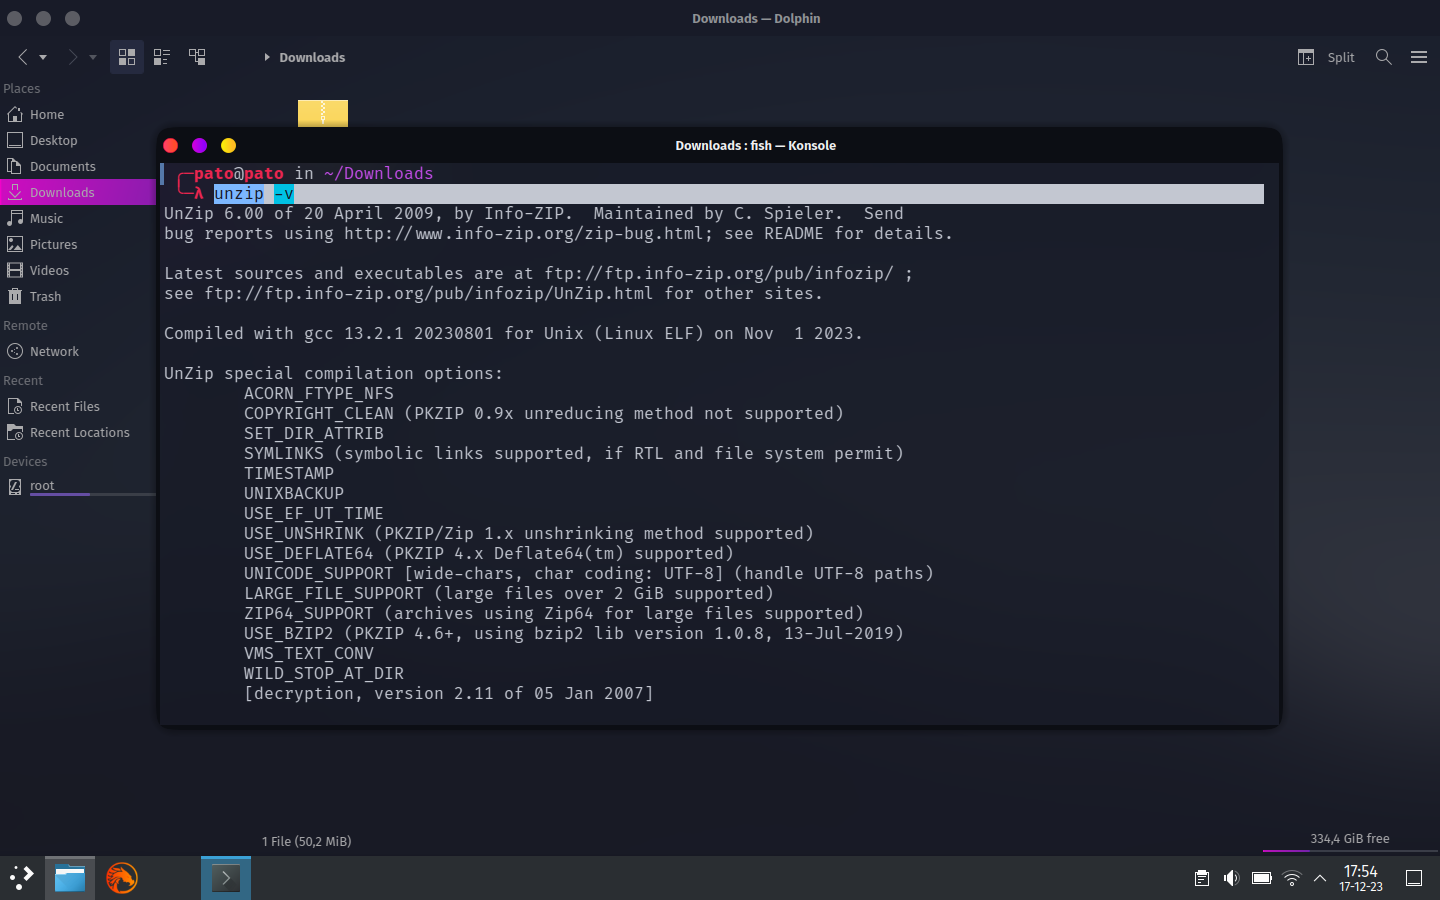
\includegraphics[width=10.5cm]{figures/TutorialLinux/tutoriallinux (4).png}
    \caption{Parte 2.2.2 Tutorial Linux}
    \label{fig:tutolinux4}
\end{figure}
\clearpage

    \item Ejecutar la descompresión del archivo usando ''unzip ./PruebaSimuladorCIMUBB-Linux.zip''.
\begin{figure}[ht]
    \centering
    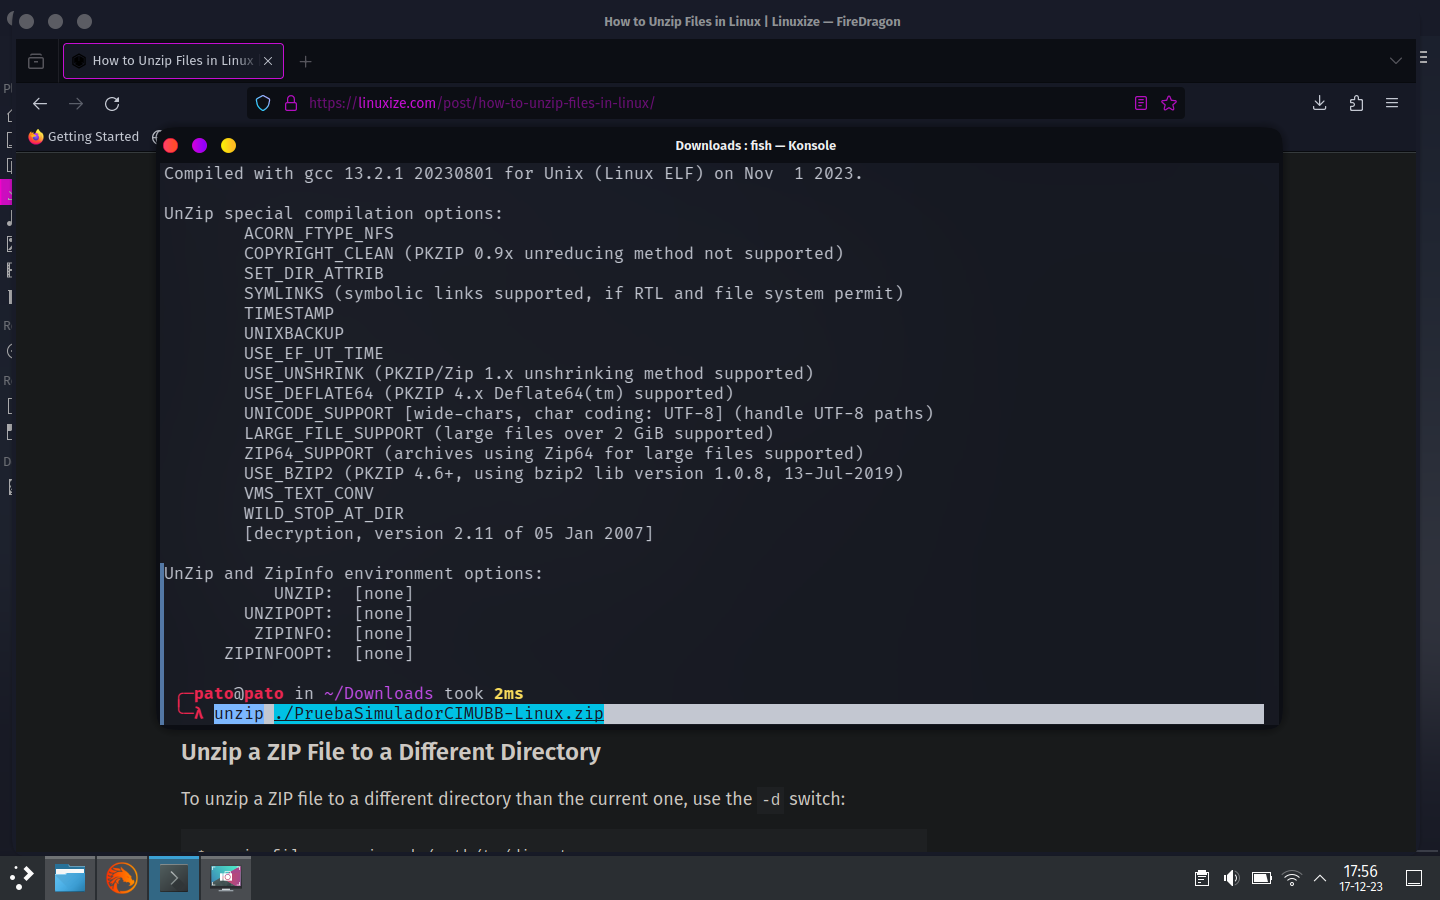
\includegraphics[width=10.5cm]{figures/TutorialLinux/tutoriallinux (5).png}
    \caption{Parte 2.2.3 Tutorial Linux}
    \label{fig:tutolinux5}
\end{figure}

    \item Abrir la carpeta extraída. De nuevo, se tienen dos opciones para realizar los siguientes pasos.
\begin{figure}[ht]
    \centering
    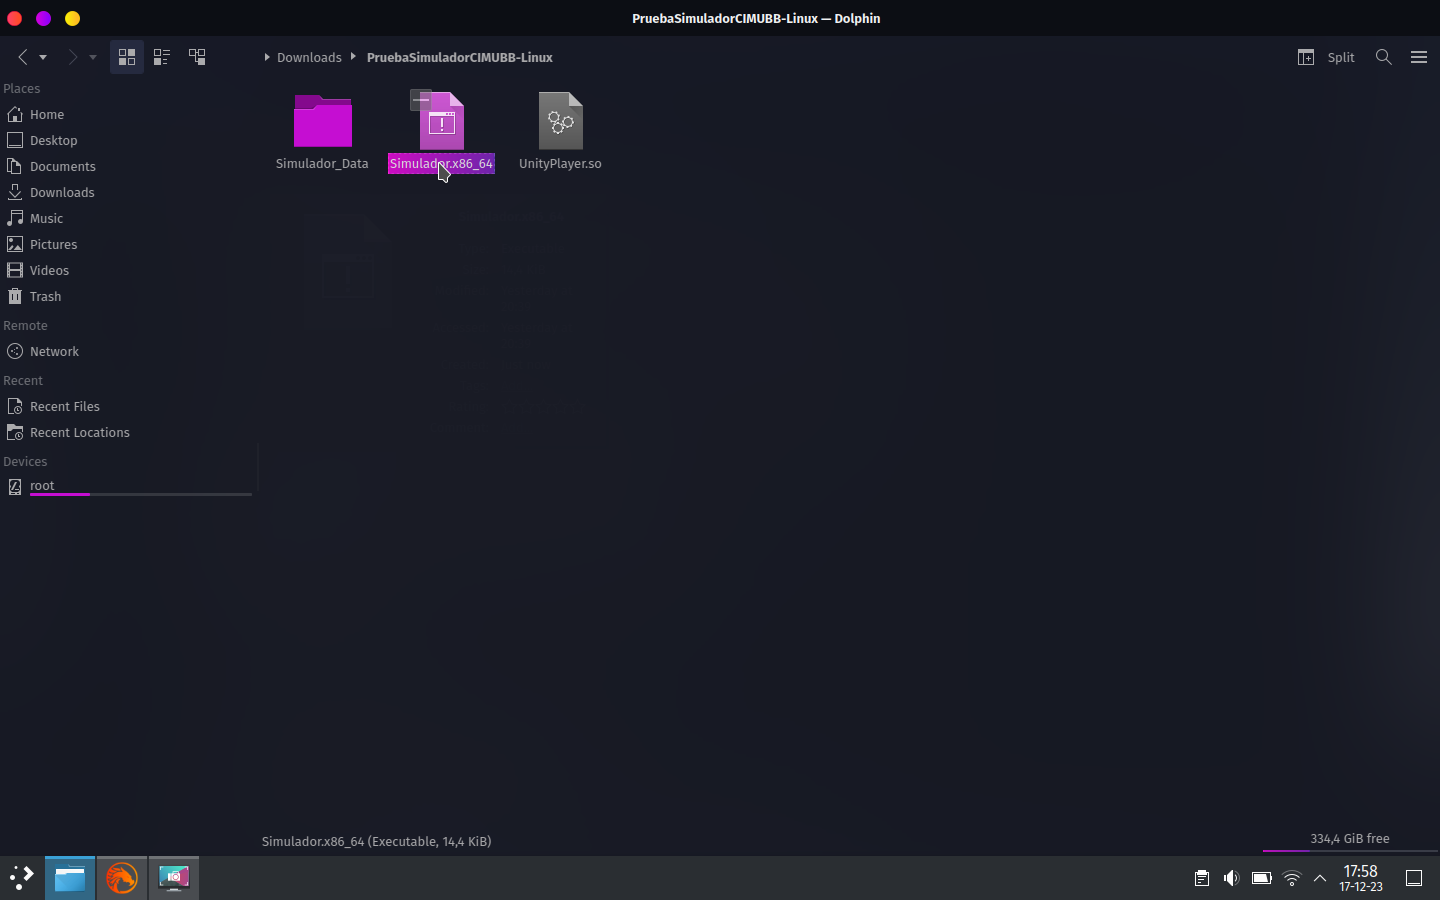
\includegraphics[width=10.5cm]{figures/TutorialLinux/tutoriallinux (6).png}
    \caption{Parte 3 Tutorial Linux}
    \label{fig:tutolinux6}
\end{figure}
\clearpage

    \item Hacer click derecho, ir a la opción ''Propiedades''.
\begin{figure}[ht]
    \centering
    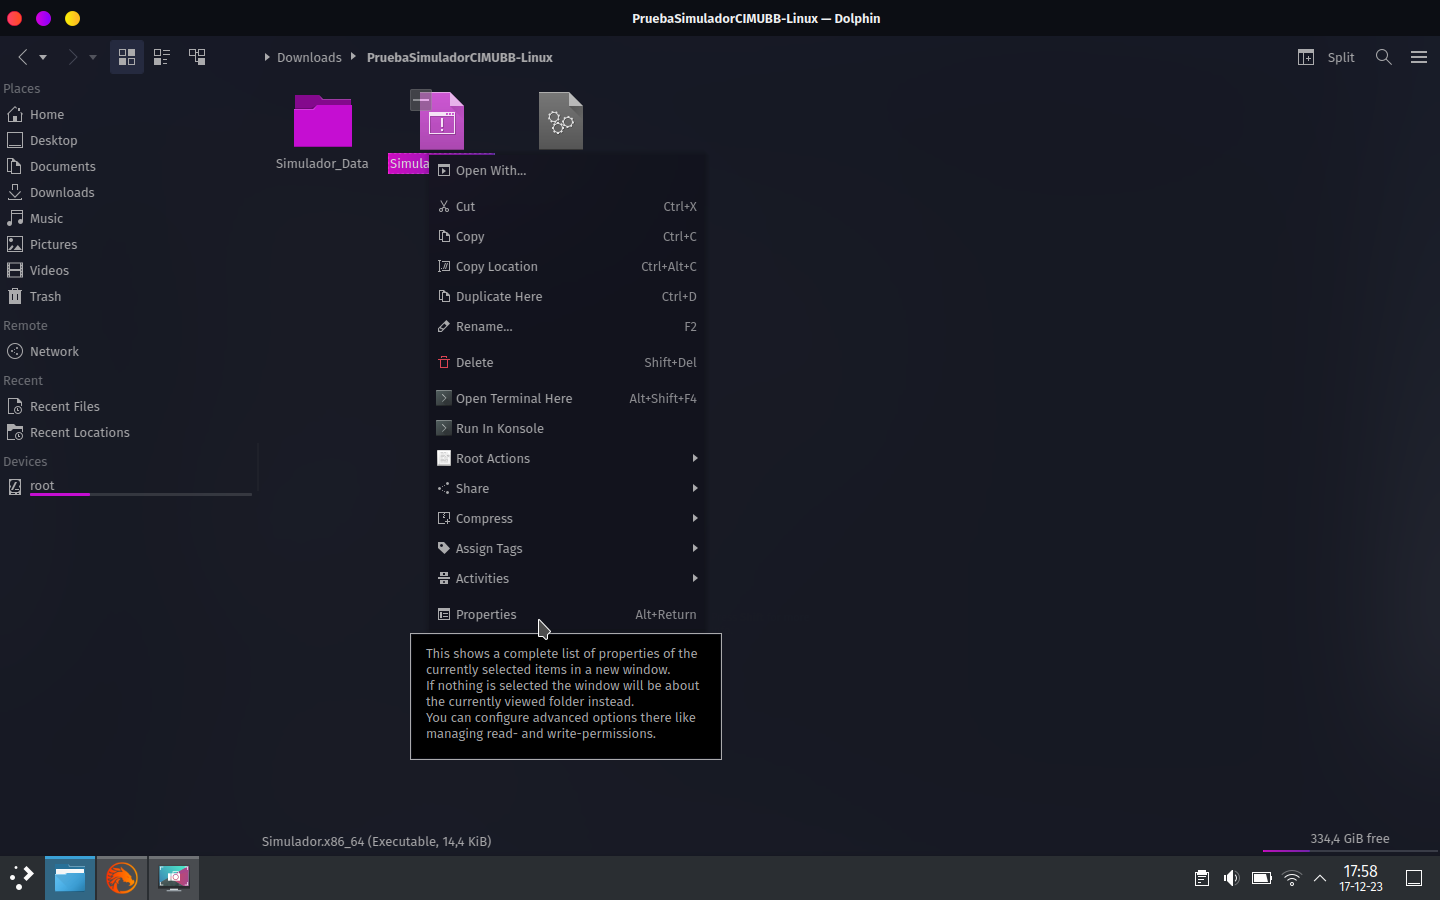
\includegraphics[width=10.5cm]{figures/TutorialLinux/tutoriallinux (7).png}
    \caption{Parte 4.1.1 Tutorial Linux}
    \label{fig:tutolinux7}
\end{figure}

    \item Ir a la pestaña ''Permisos'' y activar la casilla ''Ejecutable''.
\begin{figure}[ht]
    \centering
    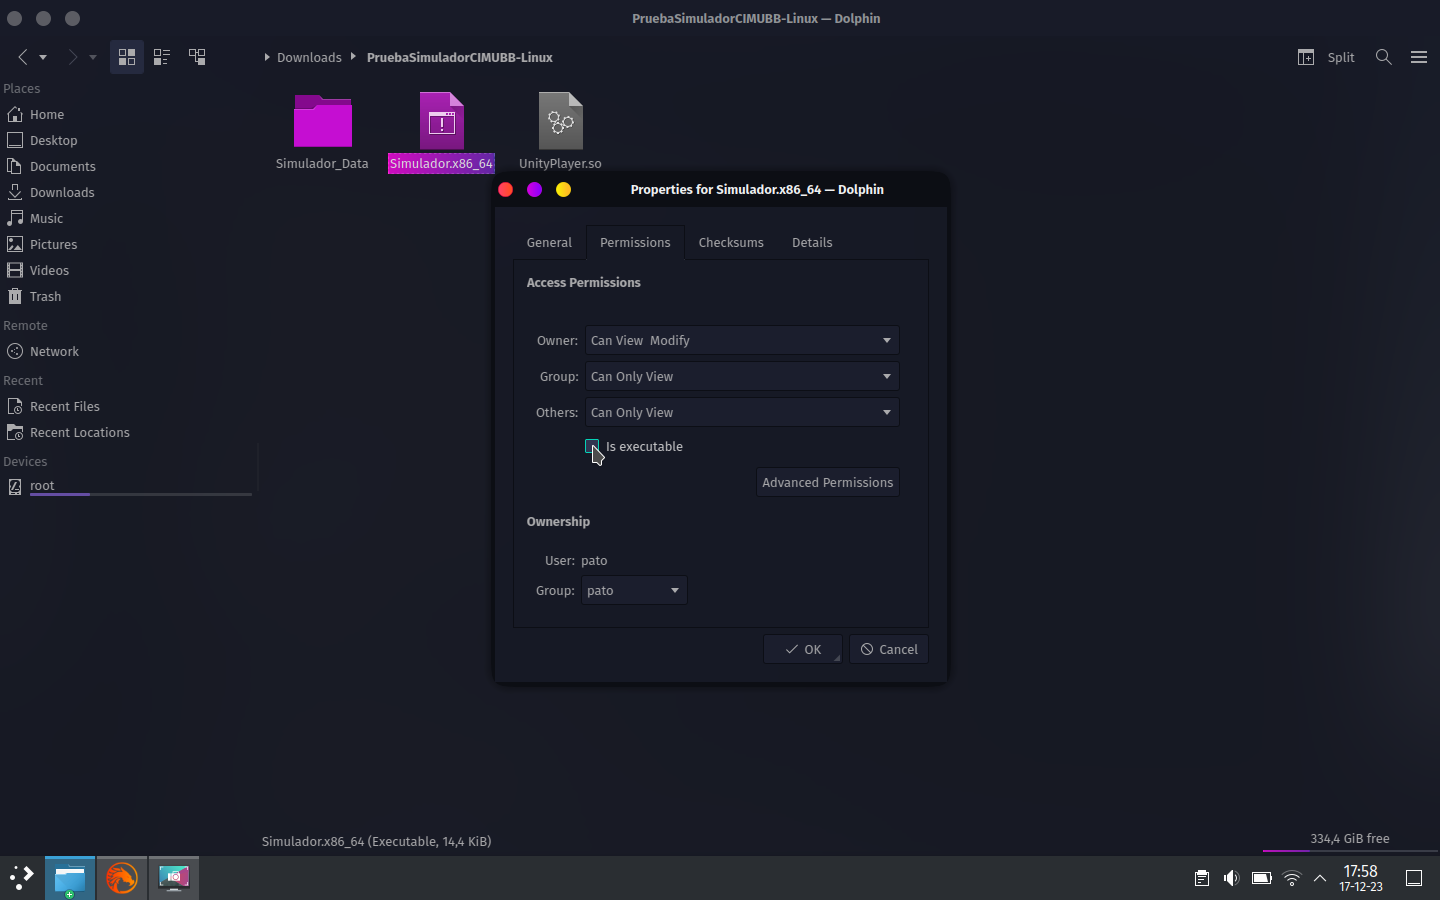
\includegraphics[width=10.5cm]{figures/TutorialLinux/tutoriallinux (8).png}
    \caption{Parte 4.1.2 Tutorial Linux}
    \label{fig:tutolinux8}
\end{figure}
\clearpage

    \item Como otra opción, en la consola usar ''chmod +x ./Simulador.x86\_64''
\begin{figure}[ht]
    \centering
    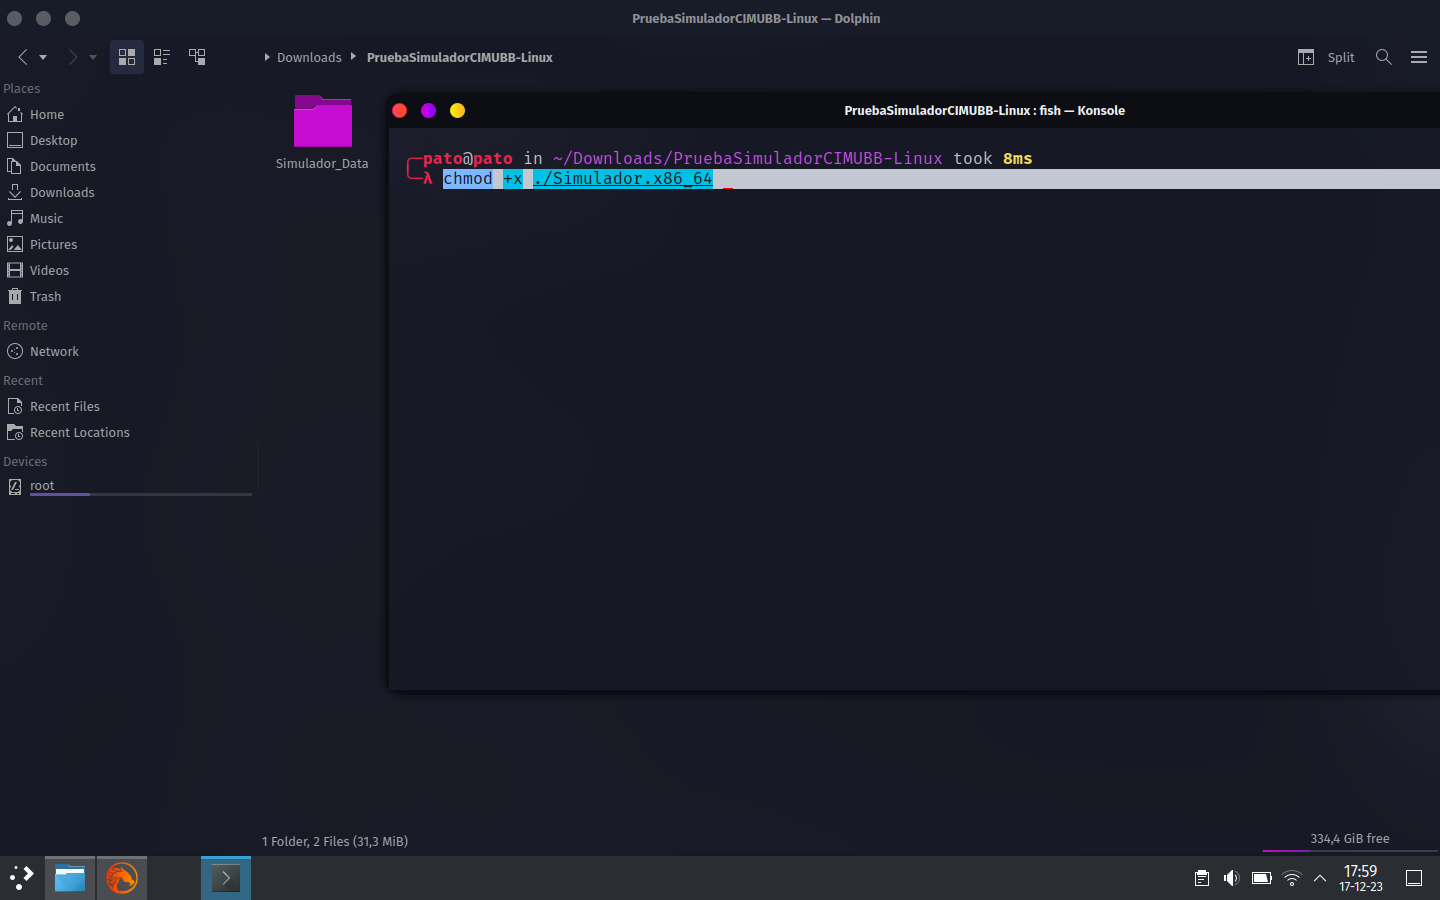
\includegraphics[width=10.5cm]{figures/TutorialLinux/tutoriallinux (9).png}
    \caption{Parte 4.2 Tutorial Linux}
    \label{fig:tutolinux9}
\end{figure}
\end{enumerate}

